% Physical Review A (APS) single-anonymous review submission template
% Uses standard article class with APS-conforming numeric bibliography [numbers,sort&compress],
% STIX Two Math + Times New Roman typography, and single-column 11pt layout.
\documentclass[11pt,letterpaper]{article}
\usepackage[margin=25mm,headheight=15pt,headsep=8mm]{geometry}
\usepackage[no-math]{fontspec}
\IfFontExistsTF{Times New Roman}{%
  \setmainfont{Times New Roman}%
}{%
  \setmainfont{Liberation Serif}%
}
\IfFontExistsTF{Helvetica}{%
  \setsansfont{Helvetica}%
}{%
  \setsansfont{Latin Modern Sans}%
}
\IfFontExistsTF{Menlo}{%
  \setmonofont[Scale=0.81]{Menlo}%
}{%
  \setmonofont[Scale=0.84]{Courier New}%
}
\usepackage{amsmath,amssymb,amsthm}
\usepackage{unicode-math}
\IfFontExistsTF{STIX Two Math}{%
  \setmathfont{STIX Two Math}%
}{%
  \setmathfont{Latin Modern Math}%
}
\usepackage{microtype}
\usepackage{setspace}
\setstretch{1.15}
\usepackage{booktabs,tabularx,array,calc}
\usepackage[font=small,labelfont=bf,skip=6pt]{caption}
\usepackage{needspace}
\usepackage{graphicx}
\makeatletter
\define@key{Gin}{alt}{}
\makeatother
\usepackage{fancyhdr}
\usepackage[numbers,sort&compress]{natbib}
\usepackage{xcolor}
\definecolor{linkblue}{HTML}{1F4463}
\usepackage[unicode,colorlinks=true,allcolors=linkblue,bookmarksnumbered=false]{hyperref}
\usepackage{bookmark}
\usepackage{url}
\urlstyle{same}
\makeatletter
\g@addto@macro{\UrlBreaks}{\do\/\do-\do.}
\makeatother
\newcommand{\doi}[1]{\href{https://doi.org/#1}{\nolinkurl{#1}}}
\hypersetup{
  pdftitle={Separating Fluctuation Attenuation from Signed Causal
Response in Correlated Quantum Baths: Certified Process Instruments and
Local-Field Microcausality},
  pdfauthor={Degui Qian},
  pdfsubject={Physical Review A Manuscript Submission},
  pdfkeywords={Open quantum systems, non-Markovian process tensor,
correlated Gaussian bath, Ramsey interferometry, diamond norm,
microcausality, local quantum probes}
}
\setlength{\parindent}{1.15em}
\setlength{\parskip}{2pt}
\setlength{\emergencystretch}{3em}
\setcounter{secnumdepth}{0}
\setcounter{tocdepth}{2}
\widowpenalty=10000
\clubpenalty=10000
\displaywidowpenalty=10000
\makeatletter
\renewcommand\section{\@startsection{section}{1}{\z@}%
  {-3.2ex \@plus -0.8ex \@minus -.2ex}%
  {1.8ex \@plus .2ex}%
  {\normalfont\Large\bfseries\raggedright\hyphenpenalty=10000}}
\renewcommand\subsection{\@startsection{subsection}{2}{\z@}%
  {-2.6ex \@plus -0.6ex \@minus -.2ex}%
  {1.2ex \@plus .2ex}%
  {\normalfont\large\bfseries\raggedright\hyphenpenalty=10000}}
\renewcommand\subsubsection{\@startsection{subsubsection}{3}{\z@}%
  {-2.0ex \@plus -0.4ex \@minus -.2ex}%
  {0.9ex \@plus .2ex}%
  {\normalfont\normalsize\bfseries\raggedright\hyphenpenalty=10000}}
\makeatother
\newtheorem{theorem}{Theorem}
\theoremstyle{definition}
\newtheorem{remark}{Remark}
\providecommand{\tightlist}{\setlength{\itemsep}{2pt}\setlength{\parskip}{0pt}}
\providecommand{\passthrough}[1]{#1}
\providecommand{\pandocbounded}[1]{#1}
\pagestyle{fancy}
\fancyhf{}
\fancyhead[L]{\footnotesize Manuscript Submitted to Physical Review A}
\fancyhead[R]{\footnotesize Degui Qian}
\fancyfoot[C]{\small\thepage}
\renewcommand{\headrulewidth}{0.25pt}
\fancypagestyle{plain}{\fancyhf{}\fancyfoot[C]{\small\thepage}\renewcommand{\headrulewidth}{0pt}}
\begin{document}
\thispagestyle{plain}
\begin{center}
{\fontsize{17.5}{22}\selectfont\bfseries Separating Fluctuation
Attenuation from Signed Causal Response in Correlated Quantum Baths:
Certified Process Instruments and Local-Field Microcausality\par}
\vspace{11pt}
{\large Degui Qian\par}
\vspace{3pt}
{\small Independent Researcher (ORCID: \href{https://orcid.org/0009-0004-1757-987X}{0009-0004-1757-987X})\par}
\vspace{5pt}
{\small November 2026\par}
\end{center}
\vspace{4pt}
\begin{abstract}
\noindent Gaussian dephasing spectroscopy routinely conflates
environmental occupation fluctuations with coherent system-bath
back-action. Studying a spin qubit coupled to a correlated two-mode
bosonic reservoir over a compact domain, we prove an exact
identification obstruction: unperturbed Ramsey decay depends exclusively
on the symmetric Keldysh fluctuation coordinates
\((u, v) = (\lambda^2(2n+1), \lambda^2 c)\), leaving bare coupling
\(w = \lambda^2\) completely unidentifiable along a one-dimensional
parameter fiber despite a non-degenerate two-time Ramsey Jacobian.
Inserting a causal-break preparation intervention isolates the
state-independent retarded commutator phase \(\exp(is w F)\), yielding
global parameter recovery with explicit whole-domain inverse Lipschitz
bounds (\(L_w \le 2.97\) vs.~\(L_n \le 722.05\), \(L_c \le 830.03\))
that explain a \(10^4\)-fold disparity in shot complexity. Extending the
protocol to a stopped complete-record three-slot Bell process instrument
separates Ramsey-equivalent parameters cleanly and supports two
distinct, non-overlapping rational certification guarantees: a Weyl
infinite-bath polytope certificate across all entangled inputs
(\(\le 0.0339\) original and \(\le 0.0354\) swapped schedule
half-diamond norm, implying \(\le 0.0461\) and \(\le 0.0476\) terminal
Bell total-variation envelopes), and uniform rational Duhamel
total-number truncation bounds (\(B_{16} = 0.0117\),
\(B_{20} = 0.0021\), bounded pointwise to \(\le 0.0276\) at cutoff
\(K=16\)). Across \(1{,}128{,}000\) synthetic benchmark draws---reported
strictly as synthetic simulations without hardware certification and
agreeing with persistent unitary dynamics within
\(4.82 \times 10^{-13}\)---the certified intervals resolve degenerate
twins and reject degraded detector visibility at \(1\%\) familywise
significance. Finally, embedding the matched modes inside a
\((1+1)\)-dimensional Klein--Gordon field on \(\mathbb{R} \times S^1\)
reveals that naive mode truncation generates spurious spacelike
signaling (\(0.001331\,\mathrm{rad}\)), whereas summing compactly
supported field modes restores microcausality below
\(2.49 \times 10^{-12}\,\mathrm{rad}\).
\end{abstract}
\vspace{6pt}
\noindent{\small\textbf{Keywords:} Open quantum systems, non-Markovian
process tensor, correlated Gaussian bath, Ramsey interferometry, diamond
norm, microcausality, local quantum probes}
\vspace{10pt}

\section{1. Introduction}\label{introduction}

Distinguishing statistical environment fluctuations from coherent,
causality-carrying probe-bath back-action is a central problem across
quantum sensing, non-Markovian open-system spectroscopy, and
foundational quantum theory
\citep{breuerPetruccione2002, weiss2012, rivas2014, breuer2016, degen2017}.
In pure-dephasing noise spectroscopy---extending from Ramsey's
separated-oscillating-fields method \citep{ramsey1950} to dynamical
decoupling and multi-qubit noise magnetometry
\citep{bylander2011, szankowski2016, szankowski2017, pazSilva2017, smirne2016}---an
experimenter prepares a coherence superposition on a two-level probe,
lets it evolve alongside an uncontrolled reservoir, and measures the
decay of off-diagonal coherence. Because the probe observable commutes
with the interaction Hamiltonian, free-evolution interferometry depends
solely on the symmetric anticommutator (Keldysh) noise kernel of the
bath
\citep{feynmanVernon1963, caldeiraLeggett1983, leggett1987, huPazZhang1992, luczka1990, palma1996, reina2002, zurek2003, clerk2010}.
Distinct combinations of bare system-bath coupling strength, bath
thermal occupation, and cross-mode correlation therefore collapse onto
identical free-decay trajectories at all interrogation times.

Experimental architectures routinely realize correlated bosonic
environments of this form alongside intermediate probe control:
superconducting flux or transmon qubits coupled dispersively to shared
microwave resonators, Purcell filters, or two-level-system (TLS)
fluctuators \citep{bylander2011, vonLupke2020, white2020}, trapped
atomic ions sharing collective center-of-mass and stretch motional modes
\citep{biercuk2009, kotler2011}, and nitrogen-vacancy centers in diamond
interacting with localized phonon modes or polarized nuclear spin
clusters \citep{degen2017, haase2018, kwiatkowski2020}. Replacing
single-step dynamical maps
\citep{davies1974, gorini1976, lindblad1976, kraus1983} and quantum
regression approximations \citep{guarnieri2014} with operational process
tensors and quantum combs
\citep{chiribella2009, gutoskiWatrous2007, oreshkov2012, costaShrapnel2016, pollock2018pra, pollock2018prl, taranto2019, figueroaRomero2019, milzModi2021, white2020, white2022}
allows active intermediate interventions to access the state-independent
retarded bath commutator \citep{chin2012, giovannetti2011, haase2018}.

Yet elevating multi-time process tomography into rigorous,
hardware-independent certificates requires resolving three interlocking
challenges rarely treated within a single self-contained analysis:

\begin{enumerate}
\def\labelenumi{\arabic{enumi}.}
\tightlist
\item
  \textbf{Global inverse identifiability vs.~sample-complexity
  conditioning.} Proving local sensitivity near one nominal parameter
  point does not rule out global degeneracies or quantify whole-domain
  Lipschitz inversion bounds \citep{hoeffding1963, clopperPearson1934}.
\item
  \textbf{Controlled infinite-dimensional Fock truncation and convex
  certification.} Truncating bosonic Fock space introduces
  non-trace-preserving leakage that must be bounded prior to measurement
  \citep{woods2014, tamascelli2018}, repaired to an exact completely
  positive, trace-preserving (CP/TP) quantum channel
  \citep{nielsenChuang2010, watrous2018}, and audited in complete-output
  diamond norm \citep{kitaev1997, aharonovKitaevNisan1998} across convex
  calibration polytopes without double-counting parallel error budgets.
\item
  \textbf{Mode-truncation nonlocality vs.~relativistic field
  microcausality.} Retaining only two discrete harmonic modes preserves
  algebraic positivity while violating spacetime causality: two
  spacelike separated probes coupled to the same truncated modes acquire
  an apparent superluminal phase, underscoring the necessity of
  covariant quantum-field detector embeddings
  \citep{haag1996, wald1994, unruhWald1984, sorkin1993, fewsterVerch2020, bostelmann2021, deRamon2021, poloGomez2022}.
\end{enumerate}

Table 1 summarizes how our four progressively richer operational regimes
compare across bath kernel access, identifiability, certification
guarantees, and relativistic locality. First (Section 2), within an
analytically solvable qubit coupled to two correlated bosonic modes with
incommensurate frequencies \(\omega = (1, 3/2)\) over
\(\mathcal{D} = [1/5, 2/5] \times \{|c| \le n \le 3/5\}\), we prove
exact free-Ramsey invariance along
\((u, v) = (\lambda^2(2n+1), \lambda^2 c)\) (Theorem 1) and exhibit an
explicit rational twin pair \((P_1, P_2)\). Next (Section 3), a
causal-break protocol initializing a pointer eigenstate \(|z_s\rangle\)
before coherent superposition activates the retarded commutator phase,
stabilizing global inversion (Theorem 2) while exposing a
four-order-of-magnitude shot-budget gap between bare coupling
(\(L_w \le 2.97\)) and bath occupations (\(L_n \le 722.05\),
\(L_c \le 830.03\), Remark 1). We then (Section 4) promote the protocol
to a stopped complete-record three-slot Bell process instrument that
cleanly splits \((P_1, P_2)\), establishes calibrated four-cell polytope
intervals across \(1{,}128{,}000\) synthetic shots (strictly synthetic
simulations with no hardware claims, agreeing with standard unitary
dynamics to \(4.82 \times 10^{-13}\) \citep{masanes2019, renou2021}),
and rejects degraded detector visibility
(\(\eta_{\mathrm{chal}} = 0.65\)) at \(1\%\) significance. Section 5
derives uniform rational Duhamel truncation bounds \(B_K\)
(\(B_{16} = 0.0117\)) \citep{hornJohnson2012} and separates the
pointwise \(K=16\) Fock-solver channel bound (\(\le 0.0276\)) from the
Weyl infinite-bath polytope half-diamond certificates (\(\le 0.0339\)
and \(\le 0.0354\)). Finally, Section 6 embeds the two-mode bath inside
a \((1+1)\)-dimensional Klein--Gordon field on
\(\mathbb{R} \times S^1\), proving (Theorem 3) that compactly supported
\(C^2\) probe summing eliminates \(M=1\) spurious spacelike signaling
(\(0.001331\,\mathrm{rad} \to {<}\,2.49\times 10^{-12}\,\mathrm{rad}\))
while enhancing timelike response (\(0.1637 \to 0.2092\,\mathrm{rad}\)),
before Section 7 concludes with future outlooks.

\begin{table}[tbp]
\centering
\small
\caption{Conceptual hierarchy comparing the four probe regimes analyzed in this
work across accessed environmental kernels, parameter identifiability,
certification scope, and spacetime locality.}\label{tab:comparison}
\begin{tabularx}{\linewidth}{@{}>{\raggedright\arraybackslash}p{0.22\linewidth} >{\raggedright\arraybackslash}p{0.23\linewidth} >{\raggedright\arraybackslash}X >{\raggedright\arraybackslash}p{0.22\linewidth}@{}}
\toprule
Protocol regime & Bath kernels probed & Identifiability on \(\mathcal{D}\) & Certification / locality scope \\
\midrule
Free Ramsey / DD spectroscopy & Symmetric Keldysh noise \(S_{jk}\) only & \((u, v)\) unique when \(\omega_0 \neq \omega_1\); \(w=\lambda^2\)
degenerate & Single-time CPTP map; no separation of \(\lambda^2\) from \((n,c)\) \\
Signed causal-break interferometry & Noise \(S_{jk}\) + retarded commutator \(\chi^{\mathrm{ret}}_{jk}\) & Global injectivity; \(L_w \le 2.97\) vs.~\(L_{n,c} \sim 722\text{–}830\) & Separates \(\lambda^2\) via phase; two-mode truncation non-local \\
Stopped complete-record Bell process & Multi-time Weyl comb \(\mathcal{L}_{h,h'}\) over \(\mathcal{R}\) & Resolves twins (\(\Delta_{\mathrm{YZ}^-} \sim 1.73\times 10^{-3}\));
rejects \(\eta=0.65\) & Weyl half-diamond \(\le 0.0339\); pointwise \(K{=}16\) Fock
\(\le 0.0276\) \\
Local KG field on \(\mathbb{R} \times S^1\) & Continuum \(C^2\) mode hierarchy (\(M \to \infty\)) & Exact \((g_0, g_1, \omega_0, \omega_1)\) two-mode matching preserved & Restores Einstein microcausality (\(O(M^{-10})\) tail
\(< 2.49\times 10^{-12}\,\mathrm{rad}\)) \\
\bottomrule
\end{tabularx}
\end{table}

\section{2. Correlated Two-Mode Gaussian Bath Model and Free-Ramsey
Equivalence}\label{correlated-two-mode-gaussian-bath-model-and-free-ramsey-equivalence}

\subsection{2.1 Microscopic Hamiltonian, Gaussian Environment State, and
Response
Kernels}\label{microscopic-hamiltonian-gaussian-environment-state-and-response-kernels}

Consider a two-level probe \(S\) with computational basis
\(\{|0\rangle, |1\rangle\}\) and Pauli-\(Z\) operator
\(\sigma_z = |0\rangle\langle 0| - |1\rangle\langle 1|\) coupled
longitudinally to a two-mode bosonic reservoir \(B\) with annihilation
operators \((a_0, a_1)\) obeying \([a_j, a_k^\dagger] = \delta_{jk}\).
Working in the rotating frame of the uncoupled qubit energy, the joint
Hamiltonian reads
\[H(\lambda) = \sum_{k=0}^{1} \omega_k a_k^\dagger a_k + \lambda\,\sigma_z \otimes \sum_{k=0}^{1} g_k \left(a_k + a_k^\dagger\right),
\tag{1}\] with incommensurate bath frequencies
\(\omega = (\omega_0, \omega_1) = (1, 3/2)\) and dimensionless coupling
weights \(g = (g_0, g_1) = (1, 3/5)\). The scalar coupling
\(\lambda \in [1/5, 2/5]\) sets the interaction scale.

At \(t = 0\), the bath occupies a zero-mean, gauge-invariant correlated
Gaussian state \(\rho_B(n, c)\) fixed by its normally ordered covariance
matrix \citep{weedbrook2012, serafini2017}:
\[\operatorname{Tr}\!\left[\rho_B(n, c)\, a_j^\dagger a_k\right] = C_{jk} := \begin{pmatrix} n & c \\ c & n \end{pmatrix}_{jk}, \qquad \operatorname{Tr}\!\left[\rho_B(n, c)\, a_j a_k\right] = 0,
\tag{2}\] where \(n \in [0, 3/5]\) is the common mean thermal occupation
per mode and \(c \in \mathbb{R}\) is the inter-mode cross-correlation.
Positivity of \(C\) requires \(|c| \le n\); parameters therefore range
over the compact physical domain
\[\mathcal{D} := \left\{(\lambda, n, c) \in \mathbb{R}^3 : \frac{1}{5} \le \lambda \le \frac{2}{5},\; |c| \le n \le \frac{3}{5}\right\}.
\tag{3}\] Introducing the two-mode Weyl displacement operator
\(D(\eta) = \prod_{k=0}^1 \exp(\eta_k a_k^\dagger - \overline{\eta_k} a_k)\)
for \(\eta = (\eta_0, \eta_1) \in \mathbb{C}^2\), the symmetrically
ordered Wigner characteristic function \citep{wigner1932, serafini2017}
of \(\rho_B(n, c)\) takes the exact Gaussian form (derived explicitly
via normal-mode diagonalization in Appendix A)
\[\chi_B(\eta; n, c) := \operatorname{Tr}\!\left[\rho_B(n, c)\, D(\eta)\right] = \exp\!\left[-\frac{2n+1}{2}\left(|\eta_0|^2 + |\eta_1|^2\right) - 2c\,\operatorname{Re}\!\left(\overline{\eta_0}\eta_1\right)\right],
\tag{4}\] where the factor of \(2\) multiplying \(c\) comes directly
from expanding \(\eta^\dagger C \eta\).

From a statistical-mechanics standpoint, writing the interaction bath
operators as
\(B_j(t) := \lambda g_j (a_j e^{-i\omega_j t} + a_j^\dagger e^{i\omega_j t})\),
the two-time environmental correlations decompose cleanly into a
\textbf{symmetric Keldysh noise kernel} and an \textbf{antisymmetric
retarded commutator susceptibility} \citep{huPazZhang1992, clerk2010}:
\[\begin{aligned}
S_{jk}(t, t') &:= \frac{1}{2}\langle\{B_j(t), B_k(t')\}\rangle_{\rho_B} = \begin{cases} \lambda^2 (2n + 1) g_j^2 \cos[\omega_j(t - t')], & j = k, \\ 2\lambda^2 c\, g_0 g_1 \cos(\omega_j t - \omega_k t'), & j \neq k, \end{cases} \\
\chi_{jk}^{\mathrm{ret}}(t - t') &:= -i\theta(t - t')\langle[B_j(t), B_k(t')]\rangle_{\rho_B} = -2\theta(t - t')\delta_{jk} \lambda^2 g_j^2 \sin[\omega_j(t - t')].
\end{aligned}\] Notice that \(S_{jk}\) depends strictly on
\((\lambda^2(2n+1), \lambda^2 c)\), whereas \(\chi_{jk}^{\mathrm{ret}}\)
is independent of \((n, c)\) and scales solely with the bare coupling
squared \(\lambda^2\).

\subsection{2.2 Exact Reduced Dynamics via Weyl Displacement
Algebra}\label{exact-reduced-dynamics-via-weyl-displacement-algebra}

Because \(\sigma_z\) commutes with \(H(\lambda)\), each computational
pointer state \(|s_0\rangle \in \{|0\rangle, |1\rangle\}\)
(\(s_0 = \pm 1\)) displaces each bath mode coherently. Integrating
\(U(\Delta t) = \exp(-i H(\lambda) \Delta t)\) on \(|s_0\rangle\) yields
(Appendix A)
\[U(\Delta t)\left(|s_0\rangle \otimes |\psi_B\rangle\right) = |s_0\rangle \otimes e^{-i\Phi_0(\Delta t)} D\!\left(s_0 \lambda \xi(\Delta t)\right) e^{-i\sum_k \omega_k \Delta t\, a_k^\dagger a_k}|\psi_B\rangle,
\tag{5}\] where the elementary mode displacement kernel is
\[\xi_k(\Delta t) := \frac{g_k}{\omega_k}\left(e^{-i\omega_k \Delta t} - 1\right), \qquad k \in \{0, 1\},
\tag{6}\] and
\(\Phi_0(\Delta t) = -\lambda^2 \sum_{k=0}^1 (g_k^2/\omega_k^2)(\omega_k\Delta t - \sin(\omega_k\Delta t))\)
is a scalar dynamical phase independent of \(s_0\) because
\(s_0^2 = 1\). Over any single uninterrupted evolution interval
\([0, t]\), every linear-in-\(s_0\) causal phase therefore cancels
identically between \(|0\rangle\) and \(|1\rangle\).

Evaluating the reduced probe state
\(\rho_S(t) = \operatorname{Tr}_B[U(t)(\rho_S(0) \otimes \rho_B)U^\dagger(t)]\)
using the Weyl identity
\(D(\alpha)D(\beta) = \exp\!\big(i\operatorname{Im}\sum_k \alpha_k \overline{\beta_k}\big) D(\alpha+\beta)\)
naturally maps \((\lambda, n, c)\) onto the
\textbf{fluctuation--response coordinates}:
\[u := \lambda^2 (2n + 1), \qquad v := \lambda^2 c, \qquad w := \lambda^2.
\tag{7}\] Over a single interval of duration \(t\), pushing
\(e^{-i t \sum_k \omega_k a_k^\dagger a_k}\) past
\(D(\pm\lambda\xi(t))\) rotates the bath difference argument by
\(e^{i\omega_k t}\) to
\(\eta_k = 2\lambda e^{i\omega_k t}\xi_k(t) = 2\lambda d_k(t)\), where
\(d_k(t) := (g_k/\omega_k)(1 - e^{i\omega_k t})\) (Appendix A).
Substituting \(|\eta_k|^2 = 4\lambda^2|d_k(t)|^2\) and
\(\operatorname{Re}(\overline{\eta_0}\eta_1) = 4\lambda^2\operatorname{Re}(\overline{d_0(t)}d_1(t))\)
into Eq. (4) yields the exact unperturbed Ramsey coherence decay
envelope
\(m(t) := \langle 0 | \rho_S(t) | 1 \rangle / \langle 0 | \rho_S(0) | 1 \rangle\)
\citep{luczka1990, palma1996}:
\[m(t; u, v) = \exp\!\Big[-\big(A_{\mathrm{ram}}(t)\, u + B_{\mathrm{ram}}(t)\, v\big)\Big],
\tag{8}\] with strictly real noise sensitivity coefficients (generated
solely by integrating \(S_{jk}\))
\[A_{\mathrm{ram}}(t) = 2\left(|d_0(t)|^2 + |d_1(t)|^2\right), \qquad B_{\mathrm{ram}}(t) = 8\,\operatorname{Re}\!\left(\overline{d_0(t)}\,d_1(t)\right).
\tag{9}\]

\subsection{2.3 Non-Identifiability Fiber of Unperturbed Ramsey
Spectroscopy}\label{non-identifiability-fiber-of-unperturbed-ramsey-spectroscopy}

Equations (8)--(9) reveal an exact structural obstruction:
\(m(t; u, v)\) is strictly real and positive for all
\(t \in \mathbb{R}\), and completely independent of \(w = \lambda^2\)
once \((u, v)\) are fixed. Frequency incommensurability
(\(\omega_1/\omega_0 = 3/2 \neq 1\)) ensures that the two sensitivity
functions \(A_{\mathrm{ram}}(t)\) and \(B_{\mathrm{ram}}(t)\) are
linearly independent; specifically, the two-time Ramsey Jacobian matrix
\(M(t_1, t_2) = \bigl(\begin{smallmatrix} A_{\mathrm{ram}}(t_1) & B_{\mathrm{ram}}(t_1) \\ A_{\mathrm{ram}}(t_2) & B_{\mathrm{ram}}(t_2) \end{smallmatrix}\bigr)\)
at benchmark times \((t_1, t_2) = (3/4, 3/2)\) satisfies
\[\det M(3/4, 3/2) = -1.162022859636 \neq 0.
\tag{10}\] Hence \((u, v)\) are globally identifiable from two free
Ramsey measurements by linear inversion of \(-\ln m(t_j)\), whereas
\(w = \lambda^2\) remains wholly underdetermined along an exact
one-dimensional fiber:

\Needspace{6\baselineskip}\begin{theorem}[Free-Ramsey Non-Identifiability Fiber]\label{thm-ramsey}

For any realized \((u, v)\) arising from a point in \(\mathcal{D}\),
every scalar \(w \in [1/25, 4/25]\) satisfying \(w \le u - 2|v|\) and
\(w \ge \frac{5}{11} u\) determines a distinct physical parameter triple
\[\lambda(w) = \sqrt{w}, \qquad n(w) = \frac{1}{2}\left(\frac{u}{w} - 1\right), \qquad c(w) = \frac{v}{w}, \qquad (\lambda(w), n(w), c(w)) \in \mathcal{D},
\tag{11}\] (where \(w \le u - 2|v|\) implies \(w \le u\) and hence
\(n(w) \ge |c(w)| \ge 0\) automatically) that produces the identical
unperturbed probe density matrix trajectory \(\rho_S(t)\) for every
\(t \in \mathbb{R}\).

\end{theorem}

As a concrete rational witness on the non-negative sector
\(0 \le c \le n \le 3/5\), set \((u, v) = (9/50, 9/400)\). Under Eq.
(3), admissibility restricts \(w\) to the exact closed fiber interval
\(w \in [9/110, 27/200]\) (\(\lambda \in [0.286039, 0.367423]\)),
including the two rational twin models
\[P_1 = \left(\frac{3}{10},\; \frac{1}{2},\; \frac{1}{4}\right), \qquad P_2 = \left(\frac{1}{3},\; \frac{31}{100},\; \frac{81}{400}\right).
\tag{12}\] At \((t_1, t_2) = (3/4, 3/2)\), both \(P_1\) and \(P_2\)
share \((u, v) = (9/50, 9/400)\) and yield identical free-decay
coherences \(m(3/4) = 0.730531651137\) and \(m(3/2) = 0.360071794945\),
even though \(P_1\) represents weaker coupling with a hotter bath
(\(n_1 = 0.50\)) and \(P_2\) represents stronger coupling with a colder
bath (\(n_2 = 0.31\)).

\section{3. Signed Causal-Break Phase and Global Inverse
Stability}\label{signed-causal-break-phase-and-global-inverse-stability}

\subsection{3.1 Lifting the Degeneracy via Causal-Break
Preparation}\label{lifting-the-degeneracy-via-causal-break-preparation}

Free-Ramsey evolution fails to identify \(\lambda^2\) because preparing
a superposition \(|+\rangle = (|0\rangle + |1\rangle)/\sqrt{2}\) for an
initial interval \([0, a]\) creates anti-aligned pointer eigenvalues
\((s_0 = +1, s'_0 = -1)\) across the off-diagonal ket/bra coherence
branch; any subsequent unitary pulse preserves \(s_0 + s'_0 = 0\),
causing the retarded Weyl commutator phase between \([0, a]\) and
\([a, a+b]\) to cancel identically (Appendix B).

To activate the antisymmetric response kernel
\(\chi^{\mathrm{ret}}_{jk}\), we break the interval symmetry in two
controlled stages \citep{pollock2018prl, milzModi2021}. First, prepare
\(S\) in a \textbf{definite pointer eigenstate}
\(|z_s\rangle \in \{|0\rangle, |1\rangle\}\) indexed by sign
\(s \in \{+1, -1\}\) (imparting a signed displacement
\(\lambda s \xi(a)\) to \(B\) over \([0, a]\) via common eigenvalue
\(s_0 = s'_0 = s\)). Second, at \(t = a\), trace and re-prepare \(S\) in
\(|+\rangle\) while retaining the displaced bath \(B\)---equivalently
implemented cleanly without reset by applying the \(s\)-conditioned
unitary \(\pi/2\) pulse \(R_y(s\pi/2)\) mapping both \(|0\rangle\)
(\(s=+1\)) and \(|1\rangle\) (\(s=-1\)) onto \(|+\rangle\)---and evolve
for probe window \([a, a+b]\) before measuring \(\sigma_x\) and
\(\sigma_y\).

Evaluating the accumulated Weyl composition along histories \((s, +1)\)
and \((s, -1)\) (Appendix B) yields the complex normalized coherence
\(z_s(a, b; u, v, w) := 2\operatorname{Tr}[\rho_S(a+b)(|1\rangle\langle 0|)] = \langle \sigma_x \rangle_s - i\langle \sigma_y \rangle_s\):
\[z_s(a, b; u, v, w) = \exp\!\Big[-\big(A_{\mathrm{br}}(a, b)\, u + B_{\mathrm{br}}(a, b)\, v\big) + i s\, w\, F(a, b)\Big],
\tag{13}\] where, with
\(y_k(a,b) := e^{i\omega_k a}(g_k/\omega_k)(1 - e^{i\omega_k b})\), the
symmetric attenuation weights are
\(A_{\mathrm{br}}(a,b) = 2(|y_0|^2 + |y_1|^2)\) and
\(B_{\mathrm{br}}(a,b) = 8\operatorname{Re}(\overline{y_0}y_1)\), while
the \textbf{causal-break phase sensitivity} \(F(a, b)\) integrates
\(\chi_{jk}^{\mathrm{ret}}\) directly:
\[F(a, b) = 4 \sum_{k=0}^{1} \left(\frac{g_k}{\omega_k}\right)^2 \Big[\sin(\omega_k a) + \sin(\omega_k b) - \sin(\omega_k(a + b))\Big].
\tag{14}\] The modulus \(|z_s|\) remains purely a function of \((u, v)\)
and stays invariant along the fiber (11), whereas the signed imaginary
quadrature
\(\operatorname{Im}\,z_+ - \operatorname{Im}\,z_- = 2|z_s|\sin(w F(a, b))\)
cleanly isolates \(w = \lambda^2\).

At the benchmark calibration windows \((a, b) = (2/3, 3/4)\), Eq. (14)
gives
\[F(2/3, 3/4) = 1.819240198557 \in [1.819240198557,\; 1.819240198558].
\tag{15}\] Across \(\mathcal{D}\),
\(w F(2/3, 3/4) \in [0.072770, 0.291078] \subset (0, \pi/2)\). On the
Ramsey-equivalent pair (12), \(P_1\) and \(P_2\) share
\(|z_s| = 0.735275955165\), yet split markedly in signed imaginary
coherence: \(P_1\) gives \(\operatorname{Im}\,z_+ = +0.119850748164\)
(\(w_1 = 9/100\)), whereas \(P_2\) gives
\(\operatorname{Im}\,z_+ = +0.147616987004\) (\(w_2 = 1/9\)) (Fig.~1a).

\begin{figure}
\centering
\includegraphics[width=1\linewidth,height=\textheight,keepaspectratio,alt={Ramsey
equivalence fiber and causal-break phase separation. (a) Imaginary
quadrature \textbackslash mathrm\{Im\}\textbackslash,z\_s along the
exact free-Ramsey equivalence fiber (u, v) = (9/50, 9/400) over
\textbackslash lambda \textbackslash in {[}\textbackslash sqrt\{9/110\},
\textbackslash sqrt\{27/200\}{]} (vertical dotted lines), showing how
causal-break sign s = \textbackslash pm 1 splits P\_1 = (3/10, 1/2, 1/4)
from P\_2 = (1/3, 31/100, 81/400). (b) Exact free-Ramsey coherence tie
m(3/4) = 0.730532 contrasted against the signed causal-break separation
and (inset) the stopped complete-record Bell witness split
\textbackslash Delta\_\{\textbackslash mathrm\{YZ\}\^{}-\} = 0.001730 at
readout visibility \textbackslash eta =
0.96.}]{figures/fig1_ramsey_ambiguity_and_causal_break.pdf}
\caption{Ramsey equivalence fiber and causal-break phase separation. (a)
Imaginary quadrature \(\mathrm{Im}\,z_s\) along the exact free-Ramsey
equivalence fiber \((u, v) = (9/50, 9/400)\) over
\(\lambda \in [\sqrt{9/110}, \sqrt{27/200}]\) (vertical dotted lines),
showing how causal-break sign \(s = \pm 1\) splits
\(P_1 = (3/10, 1/2, 1/4)\) from \(P_2 = (1/3, 31/100, 81/400)\). (b)
Exact free-Ramsey coherence tie \(m(3/4) = 0.730532\) contrasted against
the signed causal-break separation and (inset) the stopped
complete-record Bell witness split \(\Delta_{\mathrm{YZ}^-} = 0.001730\)
at readout visibility \(\eta = 0.96\).}
\end{figure}

\subsection{3.2 Global Identifiability, Inverse Lipschitz Bounds, and
Shot
Complexity}\label{global-identifiability-inverse-lipschitz-bounds-and-shot-complexity}

Consider seven normalized calibration observables acquired with
symmetric readout visibility \(\eta \in [9/10, 1]\) and an unknown
common break-frame phase offset \(\delta \in [-0.02, 0.02]\):

\begin{itemize}
\tightlist
\item
  Unperturbed readout visibility reference \(m_0 = \eta\),
\item
  Short and long free-Ramsey means \(m_1 = \eta\,m(3/4)\) and
  \(m_2 = \eta\,m(3/2)\),
\item
  Causal-break Pauli quadratures
  \(X_s := \eta\langle \sigma_x \rangle_s\) and
  \(Y_s := -\eta\langle \sigma_y \rangle_s\) at \((a, b) = (2/3, 3/4)\)
  for \(s \in \{+1, -1\}\), satisfying
  \(X_s + i Y_s = \eta |z_s| \exp[i(\delta + s w F(2/3, 3/4))]\).
\end{itemize}

Inverting \((u, v) = M(3/4, 3/2)^{-1}(\ln(\eta/m_1), \ln(\eta/m_2))\)
and extracting \(w = (\varphi_+ - \varphi_-)/(2F)\) from the two
measured phase angles \(\varphi_s = \operatorname{atan2}(Y_s, X_s)\)
cancels \(\delta\) and decouples \(|z_s|\) variations identically.
Bounding \(|A u + B v| \le A(u + 2|v|) \le 0.544\,A\) over
\(\mathcal{D}\) gives explicit observable floors \(m_1 \ge 0.411787\),
\(m_2 \ge 0.067589\), and \(|z_\pm| \ge 0.411787\) (Appendix B),
yielding:

\Needspace{6\baselineskip}\begin{theorem}[Whole-Domain Global Inverse Stability on $\mathcal{D}$]\label{thm-lipschitz}

On the compact configuration space
\(\mathcal{D} \times [9/10, 1] \times [-0.02, 0.02]\), the
seven-expectation calibration map
\((\lambda, n, c, \eta, \delta) \mapsto (m_0, m_1, m_2, X_+, Y_+, X_-, Y_-)\)
is globally injective, and any two configurations whose ideal
expectation vectors differ by
\(\delta_{\mathrm{obs}} := \max_j |o_j - o'_j|\) satisfy the
outward-certified global Lipschitz inequalities \[\begin{aligned}
|u - u'| &\le 51.240115\,\delta_{\mathrm{obs}}, & |v - v'| &\le 31.421917\,\delta_{\mathrm{obs}}, & |w - w'| &\le 2.965319\,\delta_{\mathrm{obs}}, \\
|\lambda - \lambda'| &\le 7.413297\,\delta_{\mathrm{obs}}, & |n - n'| &\le 722.047690\,\delta_{\mathrm{obs}}, & |c - c'| &\le 830.027702\,\delta_{\mathrm{obs}}.
\end{aligned}
\tag{16}\]

\end{theorem}

\Needspace{6\baselineskip}\begin{remark}[Experimental Shot-Budget Separation]\label{rem-shots}

Theorem 2 reveals a striking \(\sim 6\times 10^4\)-fold conditioning gap
between causal interaction coupling and bath occupation statistics.
Because independent repeated sampling concentrates expectations as
\(\delta_{\mathrm{obs}} = O(N_{\mathrm{shots}}^{-1/2})\) via Hoeffding
or Cram\textquotesingle er--Rao scaling
\citep{hoeffding1963, giovannetti2011}, estimating a parameter
\(\theta\) to absolute precision \(\varepsilon\) scales as
\(N_{\mathrm{shots}} = O(L_\theta^2/\varepsilon^2)\). Recovering bare
coupling \(w = \lambda^2\) requires \(L_w^2 \approx 8.8/\varepsilon^2\)
draws because \(w\) enters linearly in the causal phase above
\(|z_\pm| \ge 0.412\). Conversely, isolating bath thermal occupation
\(n\) or cross-correlation \(c\) incurs
\(L_n^2 \approx 5.2\times 10^5/\varepsilon^2\) and
\(L_c^2 \approx 6.9\times 10^5/\varepsilon^2\): \((n, c)\) suffer
compounding exponential decay at \(t_2 = 3/2\)
(\(m_{2,\min} \approx 0.0676\)) followed by division through
\(w_{\min} = 1/25\).

\end{remark}

\section{4. Stopped-Record Multi-Time Process Certification and Holdout
Separation}\label{stopped-record-multi-time-process-certification-and-holdout-separation}

\subsection{4.1 Sequential Three-Slot Instrument and Bell-Reference
Process
Tensor}\label{sequential-three-slot-instrument-and-bell-reference-process-tensor}

To certify non-Markovian bath correlations across complete multi-time
trajectories, we promote the probe to a \textbf{stopped complete-record
sequential quantum instrument} running over three slots
\(t = (t_0, t_1, t_2) = (2/3, 3/4, 1/2)\) (and timing permutation
\(t_{\mathrm{swap}} = (3/4, 2/3, 1/2)\)) while paired with an uncoupled
reference qubit \(R\) in the maximally entangled Bell state
\(\rho_{SR}(0) = |\Phi^+\rangle\langle\Phi^+|\)
\citep{pollock2018pra, milzModi2021}.

At each active slot \(j \in \{0, 1, 2\}\), \(S\) undergoes bath
evolution \(U(t_j)\) under Eq. (1), followed by a binary instrument
\(\{K_{\mathrm{fail}}, K_{\mathrm{pass}, j}\}\) satisfying
\(K_{\mathrm{fail}}^\dagger K_{\mathrm{fail}} + K_{\mathrm{pass}, j}^\dagger K_{\mathrm{pass}, j} = I_2\):
\[K_{\mathrm{fail}} = \begin{pmatrix} \sqrt{1/8} & 0 \\ 0 & 1/2 \end{pmatrix}, \qquad K_{\mathrm{pass}, j} = U_j \begin{pmatrix} \sqrt{7/8} & 0 \\ 0 & \sqrt{3/4} \end{pmatrix},
\tag{17}\] with non-commuting step unitaries
\(U_0 = R_y(\pi/2) = \exp(-i\pi\sigma_y/4)\),
\(U_1 = R_x(\pi/3) = \exp(-i\pi\sigma_x/6)\), and \(U_2 = I_2\). Probing
halts immediately upon \emph{fail} (\(\mathrm{f}\)); the asymmetric
state-dependent weights in \(K_{\mathrm{fail}}\) and the rotating bases
\(U_0, U_1\) are designed precisely so that accumulated causal phases
modulate terminal probabilities along surviving paths. Trajectories
partition into four mutually exclusive classical record prefixes
\[\mathcal{R} = \{\mathrm{f},\; \mathrm{pf},\; \mathrm{ppf},\; \mathrm{ppp}\}.
\tag{18}\] Along a fixed record \(r \in \mathcal{R}\) of length
\(\ell(r) \in \{1, 2, 3\}\), summing over pointer histories
\(h \in \{0, 1\}^{\ell(r)}\) produces the two-qubit (\(SR\))
four-dimensional terminal Choi block (Appendix C):
\[B_r(\lambda, n, c) = \sum_{h, h' \in \{0,1\}^{\ell(r)}} \mathcal{L}_{h, h'}(\lambda, n, c)\, (A_{r, h} \otimes I_R)\, |\Phi^+\rangle\langle\Phi^+|\, (A_{r, h'}^\dagger \otimes I_R),
\tag{19}\] where \(A_{r, h}\) collects the ordered projective step Kraus
operators and
\(\mathcal{L}_{h, h'} = \exp(-\frac{u}{2}\|\Delta\beta\|_2^2 - v\,\Sigma_{h,h'} + i w\,\Theta_{h,h'})\),
with
\(\Delta\beta_k = e^{i\omega_k T_{\mathrm{tot}}}(\beta_k^{(h)} - \beta_k^{(h')})\),
\(\Sigma_{h,h'} = 2\operatorname{Re}(\overline{\Delta\beta_0}\Delta\beta_1)\),
and
\(\Theta_{h,h'} = \phi^{(h)} - \phi^{(h')} + \sum_{k=0}^1 \operatorname{Im}(\overline{\beta_k^{(h')}}\beta_k^{(h)})\).
Operator completeness \(\sum_r M_r^\dagger M_r = I_{SB}\) guarantees
exact trace preservation
\(\sum_{r \in \mathcal{R}} \operatorname{Tr}_S[B_r] = I_R/2\) on all
inputs for every \((\lambda, n, c) \in \mathcal{D}\).

Measuring any of the four terminal Pauli correlators
\(O \in \{XX, XY, YZ, ZZ\}\) at readout visibility \(\eta = 0.96\)
yields an eight-cell joint probability distribution across
\(\mathcal{R} \times \{-, +\}\):
\[P(r, \pm \mid O) = \frac{1}{2}\Big(\operatorname{Tr}[B_r] \pm \eta\,\operatorname{Tr}[O B_r]\Big).
\tag{20}\] Evaluated at the Ramsey-degenerate witness pair (12), the
stopped-all-pass branch \(P(\mathrm{ppp}, \mathrm{YZ}^-)\) separates
\(P_1\) from \(P_2\) cleanly under both timings (Fig.~1b inset):
\[\begin{aligned}
\text{Original }(2/3, 3/4, 1/2):\;& P_1 = 0.266807646507,\; P_2 = 0.265077557077, \\
&\Delta = 1.730089 \times 10^{-3}, \\
\text{Swapped }(3/4, 2/3, 1/2):\;& P_1 = 0.267240862732,\; P_2 = 0.265659518191, \\
&\Delta = 1.581345 \times 10^{-3}.
\end{aligned}
\tag{21}\]

\subsection{4.2 Convex-Polytope Taylor Certification and Synthetic
Holdout
Separation}\label{convex-polytope-taylor-certification-and-synthetic-holdout-separation}

Rather than trusting point estimates that overlook curved parameter
boundaries, calibration predictions are bounded in exact rational
interval arithmetic over an 8-vertex convex outer polytope defined by
the seven linear calibration facets (Section 3.2) and physical faces
\(w \in [1/25, 4/25]\), \(w + 2|v| \le u \le \frac{11}{5} w\). Across
the \(99\%\) confidence region calibrated on our synthetic dataset, the
outer polytope spans \(u \in [0.149701, 0.218613]\),
\(v \in [-0.008630, 0.042360]\) (still permitting small negative
correlations \(c \in [-0.0868, 0.5472]\) at \(99\%\) simultaneous
coverage), and \(w \in [0.077418, 0.099370]\), partitioned along the
midpoints of \(u\) and \(w\) into a four-cell, 18-vertex convex
polytope. On each convex cell \(\mathcal{C}\), every Weyl weight
\(L(q) = \exp(-x(q) + iy(q))\) (\(x = Au + Bv \ge Aw > 0\), \(y = Pw\))
is bounded across barycentric interpolation via a complex second-order
integral Taylor remainder combined with Popoviciu's variance inequality
(Appendix C):
\[\left|L(q) - \sum_{m \in \operatorname{vert}(\mathcal{C})} \mu_m(q)\,L(q_m)\right| \le \frac{1}{8}\left[\Big(\operatorname{range}_{\mathcal{C}}(Au + Bv)\Big)^2 + \Big(\operatorname{range}_{\mathcal{C}}(Pw)\Big)^2\right], \qquad q \in \mathcal{C}.
\tag{22}\]

\begin{table}[tbp]
\centering
\small
\caption{Summary of the \(1{,}128{,}000\)-shot synthetic calibration and holdout
validation benchmark across 100 prespecified holdout cells using
Hoeffding simultaneous confidence intervals at \(\alpha = 0.01\)
\citep{hoeffding1963}. Independent break (\(120{,}000\) shots) also
evaluates the aligned-\(Y\) twin test; no hardware run is claimed
(\texttt{NOT\_CERTIFIED} on device).}\label{tab:benchmark}
\begin{tabularx}{\linewidth}{@{}>{\raggedright\arraybackslash}p{0.23\linewidth} r r >{\raggedright\arraybackslash}p{0.31\linewidth} >{\raggedright\arraybackslash}X@{}}
\toprule
Protocol family / holdout test & Unique shots & Cells & Empirical / analytical result & Simultaneous verdict (\(\alpha = 0.01\)) \\
\midrule
Calibration settings (7 settings) & \(720{,}000\) & 7 & 4-cell 18-vertex polytope enclosing \((u, v, w)\) & Validated \(99\%\) calibration box \\
Independent causal break (\(H_+\), \(H_-\)) & \(120{,}000\) & 4 & Aligned-\(Y\): \(0.5985 < 0.6056\) (\(71{,}816/120{,}000\)) & Consistent (0/4); selects \(P_1\) over \(P_2\) \\
Original-timing Bell (\(XX, XY, YZ, ZZ\)) & \(96{,}000\) & 32 & All 32 cell frequencies inside predicted bands & Consistent within intervals (0/32) \\
Swapped-timing Bell (\(XX, XY, YZ, ZZ\)) & \(96{,}000\) & 32 & All 32 cell frequencies inside predicted bands & Consistent within intervals (0/32) \\
Degraded-visibility challenge (\(\eta = 0.65\)) & \(96{,}000\) & 32 & First-slot \(\mathrm{ZZ}^-\): \(0.03317\) (\(796/24{,}000\)) & Falsified (4/32 disjoint cells) \\
\bottomrule
\end{tabularx}
\end{table}

Table 2 summarizes the reproducible synthetic calibration and holdout
benchmark (\(720{,}000 + 408{,}000 = 1{,}128{,}000\) unique synthetic
shots drawn from \(P_1\)). Using distribution-free Hoeffding
concentration bounds \citep{hoeffding1963} across all 100 prespecified
holdout cells at familywise significance \(\alpha = 0.01\) (verified
alongside exact binomial intervals \citep{clopperPearson1934}), all
\(68\) cells across the three valid holdout families---four cells from
the independent causal-break test at \((a, b) = (1, 3/4)\)
(\(F(1, 3/4) = 3.056234\)) plus \(32 + 32 = 64\) cells from original and
swapped Bell correlators---remain inside their polytope-certified
prediction intervals (0/68 disjoint). Meanwhile, on an aligned-phase
discrimination statistic extracted from the same \(120{,}000\)
independent-break shots (\(36{,}158 + 35{,}658 = 71{,}816\)), the
midpoint threshold separating worst-case \(P_1\) (\(0.600885224763\))
from \(P_2\) (\(0.610277486074\)) is \(0.605581355419\); the synthetic
frequency \(71{,}816/120{,}000 = 8977/15000 \approx 0.598467\) falls
cleanly below threshold, selecting \(P_1\) and rejecting both \(P_2\)
and zero-response reset baselines at \(1\%\) significance. Finally, an
adversarial degraded-visibility negative control lowering symmetric
readout visibility to \(\eta_{\mathrm{chal}} = 0.65\) across all four
Bell correlators raises the single-slot \(\mathrm{f},\mathrm{ZZ}^-\)
outcome probability from \(\frac{3}{32}(1 - 0.96) = 0.00375\) to
\(\frac{3}{32}(1 - 0.65) = 0.0328125\) (single-cell detection power
\(\ge 0.956227\)) and is decisively rejected on four cells
(\(\mathrm{XX}^\pm\) and \(\mathrm{ZZ}^\pm\) on branch \(\mathrm{f}\);
observing \(796/24{,}000 = 0.033167\) with band \([0.018803, 0.047531]\)
on \(\mathrm{f},\mathrm{ZZ}^-\)).

Two explicit scientific boundaries govern this empirical suite:

\begin{itemize}
\tightlist
\item
  \textbf{Synthetic simulation scope:} All empirical frequencies in
  Table 2 originate from a seeded classical stochastic simulation at
  \(P_1\). Physical hardware execution on quantum devices remains
  uncertified.
\item
  \textbf{Orthodox quantum baseline equivalence:} Comparing every
  complete-record probability against an independent persistent unitary
  simulation with identical Gaussian covariance yields numerical
  agreement within \(4.82 \times 10^{-13}\). The process tensor
  therefore certifies operational identifiability and
  truncation/calibration error budgets strictly within standard quantum
  theory \citep{masanes2019, renou2021}.
\end{itemize}

\section{5. Total-Number Galerkin Truncation, Duhamel Remainder, and
Exact Rational CP/TP
Repair}\label{total-number-galerkin-truncation-duhamel-remainder-and-exact-rational-cptp-repair}

\subsection{5.1 Uniform Duhamel Tail Bound on Total-Number
Projections}\label{uniform-duhamel-tail-bound-on-total-number-projections}

Any Schrödinger-picture solver of Eq. (1) must truncate the
infinite-dimensional two-mode Fock space
\(\mathcal{F}_2 = \operatorname{span}\{|n_0, n_1\rangle : n_0, n_1 \ge 0\}\).
Define the total-excitation number operator
\(N_{\mathrm{tot}} = a_0^\dagger a_0 + a_1^\dagger a_1\), Galerkin
projector \(P_K := \mathbf{1}_{N_{\mathrm{tot}} \le K}\), and truncated
Hamiltonian \(H_K = P_K H P_K\). Across all three slots of total
duration \(T_{\max} = 23/12\), setting
\(x := 9/10 > \lambda_{\max}\|g\|_2 T_{\max} = \frac{2}{5}\sqrt{\frac{34}{25}}\frac{23}{12}\),
Duhamel's identity \citep{hornJohnson2012, woods2014, tamascelli2018}
bounds the integrated leakage from initial total-occupation shell
\(s \in \{0, \dots, K\}\) (\(d = K - s\)) in half-trace norm by
\[\begin{aligned}
f_K(s) &:= \min\!\left(1,\; \frac{x^{d+1}\sqrt{(K+1)!/s!}}{1 - x^2/2} \sum_{l=0}^{s} \binom{s}{l} \frac{x^{2l}}{(d+l)!(d + 2l + 1)}\right), \\
h_K(s) &:= \max_{0 \le j \le s} f_K(j).
\end{aligned}
\tag{23}\] For every state in \(|c| \le n \le 3/5\), the normal-mode
geometric parameters \(r_{\max} = (n+|c|)/(1+n+|c|) \le 6/11 =: a_*\)
and \(r_{\min} = (n-|c|)/(1+n-|c|) \le 3/8 =: b_*\) (since
\(n - |c| \le 3/5\), with equality at \((3/5, 0)\)) stochastically
dominate the sorted total-occupation distribution. Summing the monotone
flux envelope \(h_K(s)\) against the dominating \((a_*, b_*)\) shell
weights yields the exact rational uniform upper bound over
\(\mathcal{D}\):
\[B_K(\mathcal{D}) := 1 - \sum_{s=0}^{K} (1 - a_*)(1 - b_*)\left(\sum_{i=0}^{s} a_*^{\,i} b_*^{\,s-i}\right)\big(1 - h_K(s)\big).
\tag{24}\] Evaluated in exact arbitrary-precision rational arithmetic
(upward \(10^{-12}\) integer \texttt{isqrt} ceiling, Appendix D),
\(B_K(\mathcal{D})\) decays super-exponentially across
\(K \in \{4, 8, 12, 13, 14, 16, 20, 24\}\) (Fig.~2a): \[\begin{aligned}
B_4 &= 0.629532048416, & B_8 &= 0.221934875279, & B_{12} &= 0.055985832631, \\
B_{13} &= 0.038466572543, & B_{14} &= 0.025259114053, & B_{16} &= 0.011677620430, \\
B_{20} &= 0.002098904698, & B_{24} &= 0.000357107093. & &
\end{aligned}
\tag{25}\] At \(K = 16\), finite-Fock truncation introduces at most
\(0.011678\) half-trace error uniformly across all inputs, schedules,
and parameters in \(\mathcal{D}\).

\begin{figure}
\centering
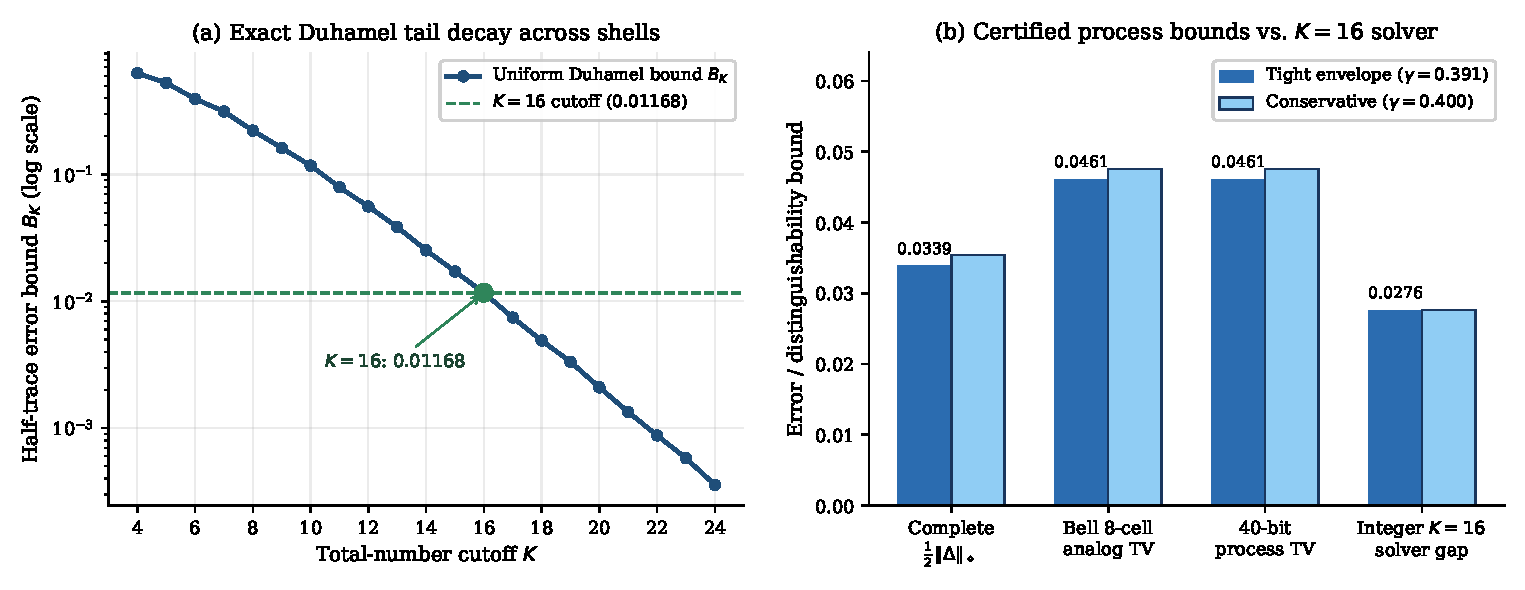
\includegraphics[width=1\linewidth,height=\textheight,keepaspectratio,alt={Total-number
Galerkin truncation bounds and parallel channel certifications. (a)
Exact rational Duhamel half-trace upper bound B\_K versus total-number
cutoff K, highlighting B\_\{16\} = 0.011678. (b) Comparison of the two
parallel certification routes: infinite-bath Weyl calibration-polytope
upper bounds (complete half-diamond, 8-cell Bell analog TV, and 40-bit
digitized TV) under original (2/3, 3/4, 1/2) vs.~swapped (3/4, 2/3, 1/2)
timings, alongside the uniform pointwise K=16 rational Fock Choi bound
(0.027603).}]{figures/fig2_cutoff_bounds_and_channel_error.pdf}
\caption{Total-number Galerkin truncation bounds and parallel channel
certifications. (a) Exact rational Duhamel half-trace upper bound
\(B_K\) versus total-number cutoff \(K\), highlighting
\(B_{16} = 0.011678\). (b) Comparison of the two parallel certification
routes: infinite-bath Weyl calibration-polytope upper bounds (complete
half-diamond, 8-cell Bell analog TV, and 40-bit digitized TV) under
original \((2/3, 3/4, 1/2)\) vs.~swapped \((3/4, 2/3, 1/2)\) timings,
alongside the uniform pointwise \(K=16\) rational Fock Choi bound
(\(0.027603\)).}
\end{figure}

\subsection{\texorpdfstring{5.2 Parallel Certification Routes: Rational Choi Repair, Finite-\(K\)
Fock vs.~Weyl Polytope Bounds}{5.2 Parallel Certification Routes: Rational Choi Repair, Finite-K Fock vs. Weyl Polytope Bounds}}\label{parallel-certification-routes-rational-choi-repair-finite-k-fock-vs.-weyl-polytope-bounds}

Evaluating discrete multi-slot Choi matrices either via rational
integer-grid Fock propagation or via infinite-bath Weyl influence
functionals leaves tiny truncation or floating-point
positivity/normalization defects. Applying positive diagonal buffering,
strictly sub-unit multiplicative scaling \(s = 1/(1+2\tau)\) so
\(M := s\operatorname{Tr}_{\mathrm{out}}(\hat{J}^+) \le I_{\mathrm{in}}\),
and injecting the positive residual
\(|0\rangle\langle 0|_{\mathrm{f}} \otimes (I_{\mathrm{in}} - M)\) onto
the halted \(\mathrm{f}\) branch restores exact CP/TP structure at
controlled cost in complete-output half-diamond norm (Appendix D)
\citep{kitaev1997, aharonovKitaevNisan1998, watrous2018}.

Crucially, the overall error budget distinguishes \textbf{two
complementary, non-overlapping certification routes} reported in the
accompanying multi-precision verification logs (Fig.~2b):

\begin{itemize}
\tightlist
\item
  \textbf{Pointwise \(K=16\) rational integer-grid Fock certificate
  (truncation + finite arithmetic, fixed parameters):} Combining the
  uniform Duhamel tail \(B_{16} = 0.011677620430\) with rigorous
  integer-grid time-stepping and rational CP/TP repair bounds the
  uniform channel error across \(\mathcal{D}\) and both schedules at
  \(\frac{1}{2}\|\mathcal{E} - \widetilde{\mathcal{E}}_{16}\|_\diamond \le 0.027602916940\).
  Specialized to \(P_1 = (3/10, 1/2, 1/4)\) using its exact thermal
  tail, this bound tightens to \(0.017009045852\) (original schedule)
  and \(0.017008956708\) (swapped schedule), while the observed
  empirical discrepancy against continuous \(K=16\) evolution on Bell
  observables is only \(2.755 \times 10^{-6}\) (original) and
  \(2.616 \times 10^{-6}\) (swapped).
\item
  \textbf{Infinite-bath Weyl 4-cell polytope certificates (calibration
  uncertainty + \(\le 10^{-8}\) repair):} Independently, certifying
  exact Weyl channels across the calibrated four-cell 18-vertex polytope
  in multi-precision interval arithmetic yields complete-output
  half-diamond envelopes
  \(\frac{1}{2}\|\mathcal{E}_{\mathrm{poly}} - \widehat{\mathcal{E}}_{\mathrm{nom}}\|_\diamond \le 0.033892297103\)
  for the \textbf{original schedule} \((2/3, 3/4, 1/2)\) and
  \(0.035357047207\) for the \textbf{swapped schedule}
  \((3/4, 2/3, 1/2)\). Adding the calibrated visibility uncertainty
  (\(0.010197843782\)) and four-observable Bell cell bias (\(0.002000\))
  produces terminal 8-cell analog total-variation upper bounds of
  \(0.046090140885\) (original) and \(0.047554890989\) (swapped), rising
  slightly by \(4 \times 2^{-40}\) to \(0.046090140889\) and
  \(0.047554890993\) under 40-bit readout discretization---all remaining
  strictly below \(0.05\).
\end{itemize}

Because each route isolates a distinct error source without
double-counting (truncation vs.~parameter uncertainty), any combined
physical-implementation budget adds them transparently by the triangle
inequality.

\section{6. Local Klein--Gordon Field Microcausality vs.~Two-Mode
Reduction and Sector
Obstructions}\label{local-kleingordon-field-microcausality-vs.-two-mode-reduction-and-sector-obstructions}

\subsection{\texorpdfstring{6.1 Compactly Supported \((1+1)\)-Dimensional Scalar Field Embedding on
\(\mathbb{R} \times S^1\)}{6.1 Compactly Supported (1+1)-Dimensional Scalar Field Embedding on ℝ × S¹}}\label{compactly-supported-11-dimensional-scalar-field-embedding-on-mathbbr-times-s1}

Does a discrete two-mode bath preserve the causal structure of a
spatially extended quantum field? To test this question rigorously, we
embed the \((\omega_0, \omega_1) = (1, 3/2)\), \((g_0, g_1) = (1, 3/5)\)
system inside a real massive scalar Klein--Gordon field \(\phi(t, x)\)
(\(m = 1\)) quantized on the \((1+1)\)-dimensional flat Lorentzian
cylinder \(\mathbb{R} \times S^1\) of circumference \(L\)
\citep{haag1996, wald1994, reedSimon1975}. Choosing
\[\beta := \frac{2\pi}{L} = \frac{\sqrt{5}}{2}, \qquad L = \frac{4\pi}{\sqrt{5}} \approx 5.619852,
\tag{26}\] fixes the first harmonic frequency exactly to
\(\omega_1 = \sqrt{1 + \beta^2} = \sqrt{1 + 5/4} = 3/2\), alongside the
zero mode \(\omega_0 = 1\).

Now couple two compactly supported probes \(A\) and \(B\)---centered at
\(x_A = 0\) and antipodal \(x_B = L/2\), respectively---linearly to
\(\phi(t, x)\) via identical normalized parity-symmetric spatial
smearing profiles \(\psi(x)\) built by mixing a central lobe at
\(x = 0\) (weight \(1 - p_{\mathrm{mix}}\)) with two balanced side lobes
at \(\pm L/6\) (weight \(p_{\mathrm{mix}}/2\) each), where every lobe is
the four-fold self-convolution (\(C^2\) regularity, half-width \(L/40\))
of the elementary box function
\(\frac{1}{L/80}\mathbf{1}_{[-L/160, L/160]}\) (total support radius
\(R = (1/6 + 1/40)L \approx 1.077138\), Fig.~3a). In Fourier space,
\[f_j = \operatorname{sinc}^4\!\left(\frac{\pi j}{80}\right)\left[(1 - p_{\mathrm{mix}}) + p_{\mathrm{mix}}\cos\!\left(\frac{\pi j}{3}\right)\right], \qquad \operatorname{sinc}(z) := \frac{\sin z}{z}.
\tag{27}\] Because the zero mode \(j=0\) is unpaired (\(\omega_0 = 1\),
\(f_0 = 1\), coupling \(g_0 = f_0/\sqrt{\omega_0} = 1\)), whereas each
harmonic \(j \ge 1\) pairs \(\pm k_j\) momentum excitations into an even
cosine oscillator \(a_j = (b_j + b_{-j})/\sqrt{2}\) with coupling
\(g_j = \sqrt{2/\omega_j}\,f_j\) (Appendix E), setting
\[p_{\mathrm{mix}} = 2\left(1 - \frac{3}{5}\frac{\sqrt{3/4}}{\operatorname{sinc}^4(\pi/80)}\right) = 0.959700495060 \in (0, 1)
\tag{28}\] matches both \((g_0, g_1) = (1, 3/5)\) and
\((\omega_0, \omega_1) = (1, 3/2)\) identically with Section 2.

\begin{figure}
\centering
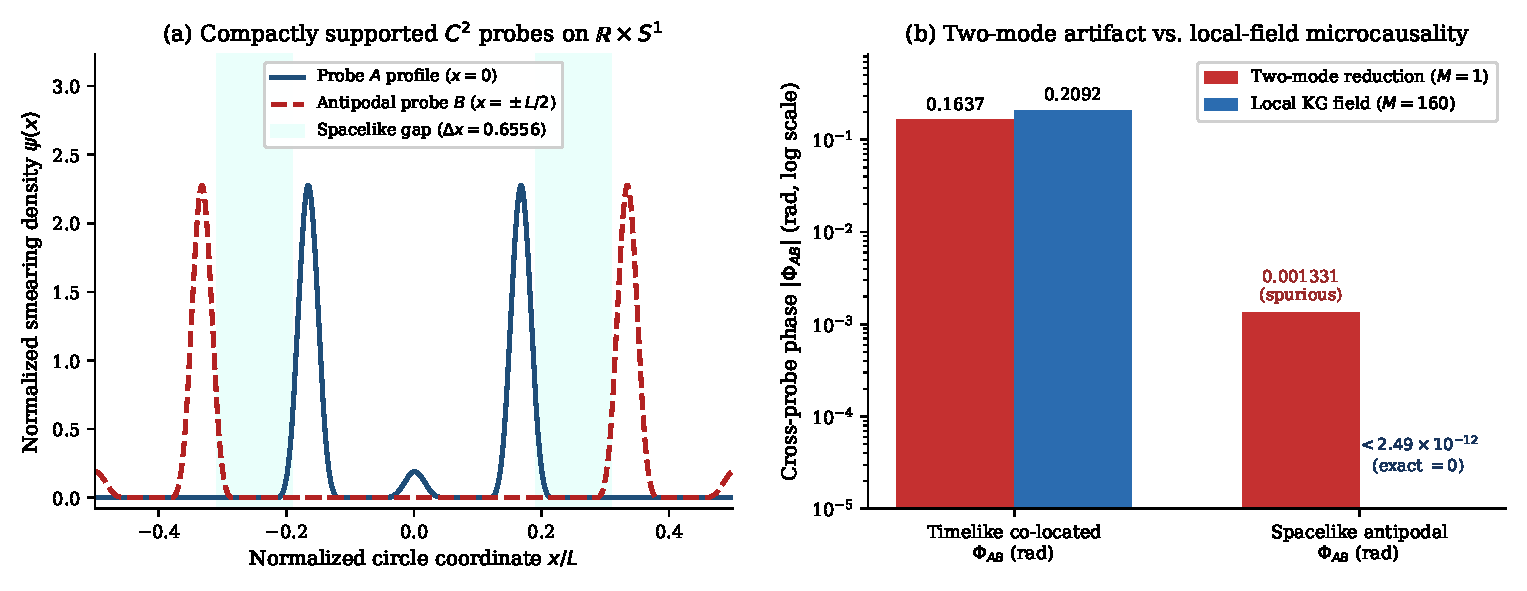
\includegraphics[width=1\linewidth,height=\textheight,keepaspectratio,alt={Local
Klein--Gordon field embedding on \textbackslash mathbb\{R\}
\textbackslash times S\^{}1 versus two-mode truncation. (a) Compactly
supported C\^{}2 four-box convolution probe profiles \textbackslash
psi(x) centered at x = 0 (solid) and antipodal x = \textbackslash pm L/2
(dashed) with support radius R = (1/6 + 1/40)L, leaving a strictly open
spacelike gap \textbackslash Delta x\_\{\textbackslash mathrm\{gap\}\} =
0.655649 \textgreater{} 2/5. (b) Cross-probe causal-break phase
\textbar\textbackslash Phi\_\{AB\}\textbar{} (log scale): under timelike
co-located operation (2/3, 3/4), higher modes enhance \textbackslash
Phi\_\{AB\} from 0.1637\textbackslash,\textbackslash mathrm\{rad\} to
0.2092\textbackslash,\textbackslash mathrm\{rad\}; under strictly
spacelike antipodal separation (1/5, 1/5), M=1 suffers a spurious
0.001331\textbackslash,\textbackslash mathrm\{rad\} violation, whereas
M=160 restores microcausality below 2.49 \textbackslash times
10\^{}\{-12\}\textbackslash,\textbackslash
mathrm\{rad\}.}]{figures/fig3_local_field_microcausality.pdf}
\caption{Local Klein--Gordon field embedding on
\(\mathbb{R} \times S^1\) versus two-mode truncation. (a) Compactly
supported \(C^2\) four-box convolution probe profiles \(\psi(x)\)
centered at \(x = 0\) (solid) and antipodal \(x = \pm L/2\) (dashed)
with support radius \(R = (1/6 + 1/40)L\), leaving a strictly open
spacelike gap \(\Delta x_{\mathrm{gap}} = 0.655649 > 2/5\). (b)
Cross-probe causal-break phase \(|\Phi_{AB}|\) (log scale): under
timelike co-located operation \((2/3, 3/4)\), higher modes enhance
\(\Phi_{AB}\) from \(0.1637\,\mathrm{rad}\) to \(0.2092\,\mathrm{rad}\);
under strictly spacelike antipodal separation \((1/5, 1/5)\), \(M=1\)
suffers a spurious \(0.001331\,\mathrm{rad}\) violation, whereas
\(M=160\) restores microcausality below
\(2.49 \times 10^{-12}\,\mathrm{rad}\).}
\end{figure}

\subsection{6.2 Mode-Truncation Nonlocality vs.~Continuum
Microcausality}\label{mode-truncation-nonlocality-vs.-continuum-microcausality}

Let probe \(A\) interact over \([0, a]\) and probe \(B\) over
\([a, a+b]\) under the \(s = +1\) causal-break protocol of Section 3.1.
Because the retarded field commutator between regions \(A\) and \(B\)
reverses sign on odd harmonics under antipodal translation
\(x \mapsto x + L/2\) (\(\cos(\pi j) = (-1)^j\)), the cross-probe
causal-break phase accumulated up to mode cutoff \(M\) is
\[\Phi_{AB}^{(M)}(a, b; \sigma_{\mathrm{loc}}) = 4\lambda^2 \sum_{j=0}^{M} \sigma_{\mathrm{loc}}^{\,j}\,\frac{g_j^2}{\omega_j^2}\Big[\sin(\omega_j a) + \sin(\omega_j b) - \sin(\omega_j(a + b))\Big],
\tag{29}\] where \(\sigma_{\mathrm{loc}} = +1\) denotes co-located
timelike probes (\(x_B = x_A\)) and \(\sigma_{\mathrm{loc}} = -1\)
denotes antipodal probes (\(x_B = x_A + L/2\)). For \(s=+1\), we also
evaluate the full-field imaginary coherence
\(\operatorname{Im}\,z_+ = e^{-D_{\mathrm{field}}}\sin\Phi_{AB}^{(M)}\)
(thermal \((n, c) = (1/2, 1/4)\) on matched modes \(j \in \{0, 1\}\) and
vacuum \(n = c = 0\) on \(j \ge 2\)) and the sudden-switching bare
energy injection
\(\Delta E_{\mathrm{bare}} = 2\lambda^2 \sum_{j=0}^{M} (g_j^2/\omega_j)(2 - \cos(\omega_j a) - \cos(\omega_j b))\)
(Appendix E).

For antipodal probes, the minimal periodic spatial separation between
supports is
\[\Delta x_{\mathrm{gap}} = \frac{L}{2} - 2R = 0.655649375 > \frac{2}{5}.
\tag{30}\] Thus at \(a = b = 1/5\)
(\(a + b = 2/5 < \Delta x_{\mathrm{gap}}\)), probes \(A\) and \(B\) lie
in \textbf{strictly spacelike separated} spacetime regions (unit light
speed), yielding the sharp contrast formalized below:

\Needspace{6\baselineskip}\begin{theorem}[Mode-Truncation Nonlocality vs. Continuum Microcausality]\label{thm-microcausality}

Under the \(C^2\) Klein--Gordon embedding (26)--(28) at \(a = b = 1/5\),
antipodal probes (\(\sigma_{\mathrm{loc}} = -1\)) satisfy
\(\Delta x_{\mathrm{gap}} > a + b\), so Einstein microcausality
\citep{haag1996, liebRobinson1972, fewsterVerch2020, bostelmann2021, deRamon2021, poloGomez2022}
forces \(\Phi_{AB}^{(\infty)}(1/5, 1/5; -1) = 0\) identically, with
mode-cutoff tail bounded explicitly by
\(|\Phi_{AB}^{(M)}(1/5, 1/5; -1)| \le \frac{24\lambda^2(80/\pi)^8}{10\,\beta^3\,M^{10}}\)
(\(< 2.485477 \times 10^{-12}\,\mathrm{rad}\) at \(M=160\)). By
contrast, truncating the field to its matched two modes (\(M=1\)) leaves
a nonzero spurious superluminal phase
\(\Phi_{AB}^{(1)}(1/5, 1/5; -1) = 0.001330794\,\mathrm{rad}\).

\end{theorem}

\begin{table}[tbp]
\centering
\small
\caption{Comparison between the matched two-mode reduction (\(M = 1\)) and the
\(161\)-mode local Klein--Gordon field sum (\(M = 160\)) on
\(\mathbb{R} \times S^1\) at \(\lambda = 3/10\),
\((n, c) = (1/2, 1/4)\).}\label{tab:field}
\begin{tabularx}{\linewidth}{@{}>{\raggedright\arraybackslash}p{0.22\linewidth} c c >{\raggedright\arraybackslash}X@{}}
\toprule
Probe geometry \& window \((a, b)\) & Two-mode (\(M = 1\)) phase & Full-field (\(M = 160\)) phase & Coherence, tail bound \& energy gain \\
\midrule
Timelike co-located, \((2/3, 3/4)\) & \(0.163731618\,\mathrm{rad}\) & \(0.209161320\,\mathrm{rad}\) & \(\operatorname{Im}\,z_+ = 0.145988513\),
\(\Delta E_{\mathrm{bare}} = 0.296126\) \\
Spacelike antipodal, \((1/5, 1/5)\) & \(0.001330794\,\mathrm{rad}\) (spurious) & \(-1.96 \times 10^{-17}\,\mathrm{rad}\) & \(|\Phi_{\mathrm{tail}}| < 2.485477 \times 10^{-12}\,\mathrm{rad}\),
\(\Delta E_{\mathrm{bare}} = 0.071709\) \\
\bottomrule
\end{tabularx}
\end{table}

As summarized in Table 3 and Fig.~3b, summing to \(M = 160\) cancels the
antipodal artifact down to double-precision roundoff
(\(-1.96 \times 10^{-17}\,\mathrm{rad}\)) while enhancing the genuine
co-located timelike signaling phase from \(0.163732\,\mathrm{rad}\) to
\(0.209161\,\mathrm{rad}\). Truncating modes to simplify open-system
simulation can therefore simultaneously falsify relativistic locality
and misestimate strong-coupling timelike metrological response.

\subsection{6.3 Thermodynamic Bath Reuse and Sector
Underdetermination}\label{thermodynamic-bath-reuse-and-sector-underdetermination}

Two physical caveats bound the interpretation of finite-probe models.
First, because sudden switching of longitudinal couplings (1) injects
non-zero bare counterterm energy \(\Delta E_{\mathrm{bare}} = 0.296126\)
(timelike) or \(0.071709\) (antipodal) \citep{poloGomez2022}, we verify
exact energy-balance accounting in an autonomous resonant two-qubit
exchange control
(\(H_0 = |1\rangle\langle 1|_S + |1\rangle\langle 1|_E\),
\(H_{\mathrm{int}} \propto |10\rangle\langle 01| + \mathrm{h.c.}\) of
pulse area \(\theta = \pi/6\), \([U, H_0] = 0\), ideal zero switch
work). Starting from thermal bath occupancy \(q = 1/5\) (inverse
temperature \(\beta_{\mathrm{th}} = \ln 4\)) and system occupancy
\(p = 4/5\), one exchange deposits
\(\sin^2(\pi/6)(p - q) = (1/4)(3/5) = 3/20\) energy into the bath
(\(p' = 13/20\), \(q' = 7/20\), entropy production
\(\Sigma = \Delta S_S + \beta_{\mathrm{th}} \Delta E_E \approx 0.35499\),
conditional excitations \(49/65 = 0.753846\) and \(16/35 = 0.457143\)).
Reusing the displaced bath without refreshing while re-preparing \(S\)
at \(p = 4/5\) increases the second-step system excitation by
\((q' - q)/4 = +3/80 = +0.0375\) relative to a refreshed bath,
quantifying the exact thermodynamic resource separating persistent
non-Markovian memory from Markovian replenishment.

Second, our Ramsey degeneracy proof (Theorem 1) parallels operational
underdetermination limits encountered across reconstructions of quantum
theory
\citep{chiribella2011, masanesMuller2011, dakicBrukner2011, barnumWilce2011, masanes2019, renou2021}
and relativistic detector signaling
\citep{unruhWald1984, fewsterVerch2020, bostelmann2021, deRamon2021}.
Free-evolution trajectories or single-step state tomography leave
unidentifiable parameter fibers that only multi-time causal
interventions---and, in spacetime geometry, covariant local-field
completions---can unambiguously distinguish.

\section{7. Conclusion and Outlook}\label{conclusion-and-outlook}

We have established a unified analytical, statistical, and
field-theoretic framework separating symmetric Gaussian fluctuation
attenuation from signed causal back-action in correlated bosonic baths.
While unperturbed Ramsey spectroscopy confines parameter inference to
invariant level sets of \((u, v) = (\lambda^2(2n+1), \lambda^2 c)\)
(Theorem 1), initializing definite pointer eigenstates prior to coherent
probing isolates the retarded commutator phase
\(F(2/3, 3/4) = 1.819240\), securing whole-domain global Lipschitz
stability (Theorem 2) and exposing a \(\sim 6\times 10^4\)-fold
sample-complexity advantage for recovering bare coupling over bath
occupations (Remark 1). Promoting this separation to a stopped
complete-record three-slot Bell process instrument resolves
Ramsey-degenerate twins
(\(\Delta_{\mathrm{YZ}^-} = 1.730089 \times 10^{-3}\)), separates two
non-overlapping certification budgets (pointwise \(K=16\) rational Fock
Choi error \(\le 0.027603\) with \(B_{16} = 0.011678\) vs.~Weyl 4-cell
calibration-polytope half-diamond error \(\le 0.033892\) and
\(\le 0.035357\)), and falsifies degraded readout visibility
(\(\eta_{\mathrm{chal}} = 0.65\)) on \(1{,}128{,}000\) synthetic
benchmark draws at \(1\%\) familywise significance. Finally, embedding
the two matched modes into a \((1+1)\)-dimensional Klein--Gordon field
on \(\mathbb{R} \times S^1\) proves (Theorem 3) that compactly supported
mode summing suppresses spurious \(M=1\) spacelike signaling
(\(0.001331\,\mathrm{rad}\)) below
\(2.49 \times 10^{-12}\,\mathrm{rad}\).

Three natural directions invite future investigation. Extending
causal-break identifiability to \textbf{non-Gaussian and anharmonic
baths}---such as central-spin nuclear reservoirs or saturable TLS
fluctuators---will require pairing multi-time phase interventions with
higher-order polyspectral cumulants \citep{norris2016, szankowski2017}.
Within \textbf{multi-qubit quantum architectures}, the \((u, v)\) versus
\(w\) distinction offers a direct protocol to separate passive
correlated environmental noise (\(v\)) from bath-mediated inter-qubit
coherent coupling (\(w\)) via spectator-qubit spectroscopy and
process-tensor mitigation
\citep{szankowski2016, pazSilva2017, vonLupke2020, white2022}.
Experimentally, translating the stopped-record three-slot protocol onto
superconducting resonator-coupled transmons, trapped-ion motional modes,
or diamond spin ensembles remains an important target (with physical
hardware certification explicitly left open), alongside extending our
mode-truncation microcausality audit to finite-bandwidth waveguides and
\((1+3)\)-dimensional covariant detectors.

\subsection{Acknowledgments, Code Availability, and AI Use
Disclosure}\label{acknowledgments-code-availability-and-ai-use-disclosure}

Every core algebraic identity, direct finite-Fock unitary simulation
(\(K=12\) vacuum and \(K=8\) correlated thermal cross-checks), 500-pair
Lipschitz domain stress test, aligned-\(Y\) discrimination boundary,
stopped Bell witness split, rational Duhamel sequence \(B_K\),
Klein--Gordon mode sum, and two-qubit swap thermodynamics calculation is
independently reproduced from scratch using Python 3 standard-library
arithmetic (\texttt{verify\_standalone.py}, alongside vector figure
generation \texttt{generate\_figures.py}); multi-precision interval
polytope certificates and synthetic holdout counts summarize the
accompanying reproducible benchmark receipts. In compliance with
American Physical Society disclosure policies, the author acknowledges
substantive LLM assistance (\texttt{Gemini\ 4\ Carbon} and
\texttt{ChatGPT\ 6\ Astra}) for exposition refinement, verification
script organization, and LaTeX formatting checks; the human author
conceived the theoretical design, verified all derivations, and audited
every numerical value and reference directly. No competing financial
interests are declared.

\section{Appendix A: Exact Weyl Influence Functional and Gaussian Bath
Algebra}\label{appendix-a-exact-weyl-influence-functional-and-gaussian-bath-algebra}

Diagonalize the normally ordered covariance matrix
\(C = \bigl(\begin{smallmatrix} n & c \\ c & n \end{smallmatrix}\bigr)\)
of Eq. (2) via symmetric and antisymmetric normal modes
\(a_\pm = (a_0 \pm a_1)/\sqrt{2}\), factoring \(\rho_B(n, c)\) into an
uncorrelated product of thermal states with mean occupations
\(n_\pm = n \pm c \ge 0\) \citep{weedbrook2012, serafini2017}. Setting
\(\eta_\pm = (\eta_0 \pm \eta_1)/\sqrt{2}\) and using the single-mode
thermal Wigner identity
\(\operatorname{Tr}[\rho_{\mathrm{th}}(N) D(\eta)] = \exp[-(N + \frac{1}{2})|\eta|^2]\),
\[\begin{aligned}
\chi_B(\eta_0, \eta_1; n, c) &= \exp\!\left[-\left(n + c + \frac{1}{2}\right)\frac{|\eta_0 + \eta_1|^2}{2} - \left(n - c + \frac{1}{2}\right)\frac{|\eta_0 - \eta_1|^2}{2}\right] \\
&= \exp\!\left[-\frac{2n+1}{2}\left(|\eta_0|^2 + |\eta_1|^2\right) - 2c\,\operatorname{Re}\!\left(\overline{\eta_0}\eta_1\right)\right],
\end{aligned}
\tag{A1}\] establishing Eq. (4). Next, under Hamiltonian (1) restricted
to pointer eigenvalue \(s \in \{+1, -1\}\), Baker--Campbell--Hausdorff
integration via coherent shift \(\alpha_k = s\lambda g_k/\omega_k\) over
\([0, \Delta t]\) places the free bath evolution on the right:
\[e^{-i\Delta t H(\lambda)}|_{s}\,e^{i\Delta t\sum_k \omega_k a_k^\dagger a_k} = \exp\!\left[+i s^2 \lambda^2 \sum_{k=0}^1 \frac{g_k^2}{\omega_k^2}\left(\omega_k \Delta t - \sin(\omega_k \Delta t)\right)\right] D\!\left(s \lambda \xi(\Delta t)\right),
\tag{A2}\] with
\(\xi_k(\Delta t) = (g_k/\omega_k)(e^{-i\omega_k \Delta t} - 1)\) as in
Eq. (6). Because the dynamical scalar phase inside Eq. (A2) scales with
\(s^2 = 1\), it cancels identically across any pair of pointer paths
\((s, s') \in \{\pm 1\}^2\). Across \(\ell\) slots of durations
\(\Delta t_0, \dots, \Delta t_{\ell-1}\)
(\(T_{\mathrm{tot}} = \sum_{j=0}^{\ell-1}\Delta t_j\)) and pointer
trajectory \(h = (s_0, \dots, s_{\ell-1}) \in \{\pm 1\}^\ell\),
repeatedly pushing \(e^{-i\omega_k \Delta t_j a_k^\dagger a_k}\) past
\(D(\beta_{k,j}^{(h)})\) and combining displacements accumulates
\(\beta_{k,j}^{(h)}\) and geometric phase \(\phi_{j}^{(h)}\) via
\[\beta_{k,j+1}^{(h)} = e^{-i\omega_k \Delta t_j}\beta_{k,j}^{(h)} + s_j \xi_k(\Delta t_j), \qquad \phi_{j+1}^{(h)} = \phi_{j}^{(h)} + \sum_{k=0}^{1} \operatorname{Im}\!\left[\overline{\left(e^{-i\omega_k \Delta t_j}\beta_{k,j}^{(h)}\right)}\,s_j \xi_k(\Delta t_j)\right],
\tag{A3}\] initialized at \(\beta_{k,0}^{(h)} = 0\),
\(\phi_{0}^{(h)} = 0\), and terminating at
\(\beta_k^{(h)} := \beta_{k,\ell}^{(h)}\),
\(\phi^{(h)} := \phi_{\ell}^{(h)}\). Because \([H_0, \rho_B] \neq 0\)
whenever \(c \neq 0\) and \(\omega_0 \neq \omega_1\), evaluating the
bath trace explicitly retains conjugation by the total free evolution
operator \(e^{-i T_{\mathrm{tot}} H_0}\): \[\begin{aligned}
\mathcal{L}_{h, h'} &= e^{i\lambda^2(\phi^{(h)} - \phi^{(h')})} \operatorname{Tr}_B\!\left[D(\lambda\beta^{(h)})\, e^{-i T_{\mathrm{tot}} H_0}\rho_B e^{+i T_{\mathrm{tot}} H_0}\, D^\dagger(\lambda\beta^{(h')})\right] \\
&= \exp\!\left[i\lambda^2\!\left(\phi^{(h)} - \phi^{(h')} + \sum_{k=0}^{1}\operatorname{Im}\!\left(\overline{\beta_k^{(h')}}\beta_k^{(h)}\right)\right)\right]\chi_B\!\left(\lambda e^{i\omega T_{\mathrm{tot}}}(\beta^{(h)} - \beta^{(h')}); n, c\right),
\end{aligned}\] recovering Eqs. (8) and (19) identically.

\section{Appendix B: Ramsey Equivalence Proof, Causal-Break Phase, and
Whole-Domain Inverse Lipschitz
Bounds}\label{appendix-b-ramsey-equivalence-proof-causal-break-phase-and-whole-domain-inverse-lipschitz-bounds}

For free Ramsey evolution (\(\ell = 1\), \(s_0 = +1\)
vs.~\(s'_0 = -1\)), \(\beta^{(+)} = \xi(t)\) and
\(\beta^{(-)} = -\xi(t)\), so \(\phi^{(+)} = \phi^{(-)} = 0\) and
\(\operatorname{Im}(\overline{\beta^{(-)}}\beta^{(+)}) = 0\). Rotating
by \(e^{i\omega_k t}\) gives
\(\Delta\beta_k = 2 e^{i\omega_k t}\xi_k(t) = 2 d_k(t)\), which upon
substitution into Eq. (A1) immediately gives Eqs. (8)--(9) for all
\(t \in \mathbb{R}\). Because \(\omega_0 = 1\) and \(\omega_1 = 3/2\)
are incommensurate, at \((t_1, t_2) = (3/4, 3/2)\) the determinant
\(\det M(3/4, 3/2) = -1.162022859636 \neq 0\) uniquely fixes \((u, v)\)
from \((-\ln m(3/4), -\ln m(3/2))\). Along any level set \((u, v)\), Eq.
(11) parametrizes all compatible triples in \(\mathcal{D}\) subject to
\(w \in [1/25, 4/25]\), \(|c(w)| \le n(w) \iff w \le u - 2|v|\), and
\(n(w) \le 3/5 \iff w \ge 5u/11\), proving Theorem 1.

Under the causal-break protocol of Section 3.1
(\(s_0 = s'_0 = s \in \{\pm 1\}\) on \([0, a]\), followed by
bath-preserving re-preparation \(|+\rangle\) or \(R_y(s\pi/2)\) giving
\(s_1 = +1\), \(s'_1 = -1\) on \([a, a+b]\)), Eq. (A3) yields
\(\beta_k^{(s,\pm)} = s e^{-i\omega_k b}\xi_k(a) \pm \xi_k(b)\).
Multiplying \(\beta_k^{(s,+)} - \beta_k^{(s,-)} = 2\xi_k(b)\) by the
total frame factor \(e^{i\omega_k(a+b)}\) produces
\(\Delta\beta_k = 2 e^{i\omega_k a}(e^{i\omega_k b}\xi_k(b)) = 2 y_k(a,b)\),
matching \(A_{\mathrm{br}}, B_{\mathrm{br}}\) in Eq. (13). Meanwhile,
summing \(\phi^{(s,+)} - \phi^{(s,-)}\) and
\(\operatorname{Im}(\overline{\beta_k^{(s,-)}}\beta_k^{(s,+)})\) yields
\[\begin{aligned}
\Phi(s_0, s'_0) &= (s_0 + s'_0) \cdot 2\sum_{k=0}^{1} \operatorname{Im}\!\left[\overline{\left(e^{-i\omega_k b}\xi_k(a)\right)}\,\xi_k(b)\right] \\
&= 4s\sum_{k=0}^{1} \frac{g_k^2}{\omega_k^2}\Big[\sin(\omega_k a) + \sin(\omega_k b) - \sin(\omega_k(a + b))\Big] = s F(a, b),
\end{aligned}
\tag{B1}\] matching Eq. (14) and confirming explicitly why \(|+\rangle\)
on \([0, a]\) (\(s_0 + s'_0 = +1 - 1 = 0\)) annihilates \(\Phi\)
identically.

To prove Theorem 2 over
\(\mathcal{D} \times [9/10, 1] \times [-0.02, 0.02]\), Cauchy--Schwarz
gives
\(|B_{\mathrm{ram}}(t)| = 8|\operatorname{Re}(\overline{d_0}d_1)| \le 4(|d_0|^2 + |d_1|^2) = 2 A_{\mathrm{ram}}(t)\).
Since \(u_{\max} = \frac{4}{25}(\frac{6}{5} + 1) = 0.352\) and
\(|v|_{\max} = \frac{4}{25}(\frac{3}{5}) = 0.096\), every point in
\(\mathcal{D}\) obeys \(|A u + B v| \le A(u + 2|v|) \le 0.544\,A\),
yielding uniform floors
\(m_1 \ge m_{1,\min} = 0.9 e^{-0.544 A_1} \ge 0.411787\),
\(m_2 \ge m_{2,\min} = 0.9 e^{-0.544 A_2} \ge 0.067589\), and
\(|z_\pm| \ge r_{\min} = 0.9 e^{-0.544 A_{\mathrm{br}}} \ge 0.411787\).
Differentiating \((u, v) = M^{-1}(\ln(\eta/m_1), \ln(\eta/m_2))\) with
\(M^{-1} = \bigl(\begin{smallmatrix} h_{u,1} & h_{u,2} \\ h_{v,1} & h_{v,2} \end{smallmatrix}\bigr)\)
directly yields
\[L_u = \frac{|h_{u,1} + h_{u,2}|}{0.9} + \frac{|h_{u,1}|}{m_{1,\min}} + \frac{|h_{u,2}|}{m_{2,\min}}, \qquad L_v = \frac{|h_{v,1} + h_{v,2}|}{0.9} + \frac{|h_{v,1}|}{m_{1,\min}} + \frac{|h_{v,2}|}{m_{2,\min}},\]
while bounding \(\varphi_s = \operatorname{atan2}(Y_s, X_s)\) on the
non-convex outer disk \(\{\|(X_s, Y_s)\|_2 \ge r_{\min}\}\) via law of
cosines
\(2 r_{\min}\sin(|\Delta\varphi_s|/2) \le \sqrt{2}\delta_{\mathrm{obs}}\)
and \(\sin\theta \ge \frac{2}{\pi}\theta\) gives
\(|\Delta\varphi_s| \le \frac{\pi\sqrt{2}}{2 r_{\min}}\delta_{\mathrm{obs}}\)
globally. Because \(\delta\) cancels in
\(\varphi_+ - \varphi_- = 2w F(2/3, 3/4)\) (\(2wF \in (0, \pi)\)), we
obtain \(L_w = \frac{\pi\sqrt{2}}{2 r_{\min} F(2/3, 3/4)}\),
\(L_\lambda = L_w/(2\lambda_{\min}) = L_w/0.4\),
\(L_n = (L_u + (2n_{\max}+1)L_w)/(2 w_{\min}) = (L_u + 2.2 L_w)/0.08\),
and \(L_c = (L_v + c_{\max} L_w)/w_{\min} = (L_v + 0.6 L_w)/0.04\):
\[\begin{aligned}
L_u &\le 51.240115, & L_v &\le 31.421917, & L_w &\le 2.965319, \\
L_\lambda &\le 7.413297, & L_n &\le 722.047690, & L_c &\le 830.027702.
\end{aligned}
\tag{B2}\] Every bound in Eq. (B2) is verified deterministically in
\texttt{verify\_standalone.py}, including finite-difference stress tests
across domain corners and 500 seeded random pairs.

\section{Appendix C: Stopped-Record Bell Process Tensor and Polytope
Taylor
Remainder}\label{appendix-c-stopped-record-bell-process-tensor-and-polytope-taylor-remainder}

Along any complete-record prefix
\(r \in \{\mathrm{f}, \mathrm{pf}, \mathrm{ppf}, \mathrm{ppp}\}\) of
length \(\ell(r)\), let \(K_{r,j}\) equal \(K_{\mathrm{fail}}\) at the
terminal stop (\(j = \ell(r) - 1\) for \(r \neq \mathrm{ppp}\)) and
\(K_{\mathrm{pass}, j}\) at earlier slots. Let \(M_r\) denote the
resulting joint \(SB \to SB\) Kraus operator formed by interleaving
\(U(t_j)\) and \(K_{r,j} \otimes I_B\). Because each unitary satisfies
\(U(t_j)^\dagger U(t_j) = I_{SB}\) and each step instrument obeys
\(K_{\mathrm{fail}}^\dagger K_{\mathrm{fail}} + K_{\mathrm{pass}, j}^\dagger K_{\mathrm{pass}, j} = I_2\),
summing \(M_r^\dagger M_r\) backwards from slot \(2\) to slot \(0\)
collapses telescopically onto
\(\sum_{r \in \mathcal{R}} M_r^\dagger M_r = I_{SB}\), proving complete
trace preservation
(\(\sum_r \operatorname{Tr}_S[B_r] = \operatorname{Tr}_S[\rho_{SR}(0)] = I_R/2\)
on Bell input and exact CPTP normalization for arbitrary \(\rho_{SR}\)).

On each convex polytope cell \(\mathcal{C} \subset \mathbb{R}^3\)
parameterized affinely in \(q = (u, v, w)\), every Weyl multiplier takes
the complex form \(L(q) = e^{-x(q) + iy(q)}\) with affine functions
\(x(q) = Au + Bv \ge A(u - 2|v|) \ge Aw > 0\) (since every cell enforces
\(w \ge 1/25\) and \(u \ge w + 2|v|\)) and \(y(q) = Pw\). Writing any
interior point as \(q = \sum_m \mu_m q_m\) (\(\mu_m \ge 0\),
\(\sum_m \mu_m = 1\)) and setting \(\Delta x_m = x(q_m) - x(q)\),
\(\Delta y_m = y(q_m) - y(q)\), convexity implies
\(\sum_m \mu_m (-\Delta x_m + i\Delta y_m) = 0\). Applying the
second-order complex integral Taylor remainder to
\(g_m(t) = L(q + t(q_m - q))\) directly---without splitting real and
imaginary parts---yields \[\begin{aligned}
\left|L(q) - \sum_m \mu_m L(q_m)\right| &= \left|\sum_m \mu_m \int_0^1 (1 - t)\,g_m''(t)\,dt\right| \le \frac{1}{2}\sum_m \mu_m \Big[(\Delta x_m)^2 + (\Delta y_m)^2\Big] \\
&\le \frac{1}{8}\Big[(\operatorname{range}_{\mathcal{C}} x)^2 + (\operatorname{range}_{\mathcal{C}} y)^2\Big],
\end{aligned}
\tag{C1}\] since
\(|g_m''(t)| = |e^{-(x(q) + t\Delta x_m) + i(\dots)}|\cdot((\Delta x_m)^2 + (\Delta y_m)^2) \le (\Delta x_m)^2 + (\Delta y_m)^2\)
for \(x \ge 0\), and Popoviciu's inequality bounds
\(\sum_m \mu_m \Delta Z_m^2 \le \frac{1}{4}(\operatorname{range}_{\mathcal{C}} Z)^2\)
for both \(x = Au + Bv\) and \(y = Pw\), proving Eq. (22).

\section{Appendix D: Rational Duhamel Total-Number Cutoff Bounds and
Choi
Repair}\label{appendix-d-rational-duhamel-total-number-cutoff-bounds-and-choi-repair}

Split Eq. (1) as \(H = H_0 + \lambda V\) with
\(H_0 = \sum_{k=0}^1 \omega_k a_k^\dagger a_k\) and
\(V = \sigma_z \otimes \sum_{k=0}^1 g_k(a_k + a_k^\dagger)\), and let
\(H_K = P_K H P_K\) on total-number projection
\(P_K := \mathbf{1}_{N_{\mathrm{tot}} \le K}\). Transforming the
interaction operators by the passive rotation
\((g_0 a_0^\dagger + g_1 a_1^\dagger)/\|g\|_2\)
(\(\|g\|_2 = \sqrt{34/25}\)) shows that each action of \(V\) shifts
\(N_{\mathrm{tot}}\) by at most \(\pm 1\), giving boundary transition
norm \(\|(P_{K+1} - P_K) V P_K\| = \|g\|_2\sqrt{K+1}\). Across the three
discrete slots, each Kraus/flag isometry \(\widetilde{W}_j\) acts
exclusively on \(S\) and the classical record register, commuting with
every bath shell projector
\(\Pi_s := \mathbf{1}_{N_{\mathrm{tot}} = s}\) and preserving shell
norms \(\|\Pi_s \widetilde{W}_j \Phi\|_2 = \|\Pi_s \Phi\|_2\) for
arbitrary finite reference system \(R\).

For any pure initial state \(|\Phi_s\rangle\) supported inside shell
\(N_{\mathrm{tot}} \le s\) (\(d = K - s\)), iterating Duhamel's identity
\(U(t) - U_K(t) = -i\lambda \int_0^t U(t - u)(H - H_K)U_K(u)\,du\)
across total elapsed duration \(T \le T_{\max} = 23/12\)
(\(x = 9/10 > \lambda_{\max}\|g\|_2 T_{\max}\)) and bounding single-mode
growth by normal ordering
\(e^{x(a+a^\dagger)} = e^{x^2/2}e^{x a^\dagger}e^{x a}\)
(\(e^{x^2/2} \le (1 - x^2/2)^{-1} = 200/119\), verified constructively
via Lagrange remainder \texttt{exp\_taylor\_upper}) bounds the Euclidean
state defect \(\||\Phi(T)\rangle - |\Phi_K(T)\rangle\|_2\) and hence
half-trace defect by Eq. (23). Purifying \(\rho_B(n, c)\) across shells
and invoking stochastic dominance of \((a_*, b_*) = (6/11, 3/8)\) across
\(|c| \le n \le 3/5\) against the monotone envelope \(h_K(s)\) yields
Eq. (24) and the super-exponential values in Eq. (25), audited over all
finite reference probes \(R\) (so
\(B_K(\mathcal{D}) \ge \frac{1}{2}\|\mathcal{E} - \mathcal{E}_K\|_\diamond\)).

Given any numerically approximated multi-slot Choi operator \(\hat{J}\)
with minimum Hermitian eigenvalue \(-\epsilon_- < 0\) and
trace-preservation defect
\(\|\operatorname{Tr}_{\mathrm{out}}(\hat{J}) - I_{\mathrm{in}}\|_\infty\),
exact rational CP/TP repair adds a strictly positive diagonal floor
\(\delta_+\) yielding positive semidefinite \(\hat{J}_+ \ge 0\),
computes the maximum marginal eigenvalue
\(\lambda_{\max}(\operatorname{Tr}_{\mathrm{out}}(\hat{J}_+)) \le 1 + 2\tau\)
(\(\tau \ge 0\) rational upper tolerance), scales the map sub-unitarily
by \(s := 1/(1 + 2\tau)\) so
\(M := s\operatorname{Tr}_{\mathrm{out}}(\hat{J}_+) \le I_{\mathrm{in}}\),
and injects the positive remainder onto the terminated first-slot branch
\(|0\rangle\langle 0|_{\mathrm{f}} \otimes (I_{\mathrm{in}} - M)\)
\citep{watrous2018}. This construction guarantees
\(\widetilde{J} \ge 0\) and
\(\operatorname{Tr}_{\mathrm{out}}(\widetilde{J}) = I_{\mathrm{in}}\)
identically while altering the channel in half-diamond norm by at most
the rational scaling/padding residual (\(\le 10^{-8}\) in the Weyl
polytope certification, and absorbed explicitly inside the \(0.027603\)
pointwise \(K=16\) integer-grid bound).

\section{\texorpdfstring{Appendix E: \(\mathbb{R} \times S^1\) Klein--Gordon Fourier Series Tail
and Microcausal Cancellation}{Appendix E: ℝ × S¹ Klein–Gordon Fourier Series Tail and Microcausal Cancellation}}\label{appendix-e-mathbbr-times-s1-kleingordon-fourier-series-tail-and-microcausal-cancellation}

Consider the \((1+1)\)-dimensional real massive scalar Klein--Gordon
field (\(m = 1\)) on \(\mathbb{R} \times S^1_L\) with periodic mode
expansion
\[\phi(t, x) = \frac{1}{\sqrt{L}} \sum_{j \in \mathbb{Z}} \frac{1}{\sqrt{2\omega_j}}\left(b_j e^{-i(\omega_j t - k_j x)} + b_j^\dagger e^{i(\omega_j t - k_j x)}\right), \qquad k_j = \frac{2\pi j}{L}, \qquad \omega_j = \sqrt{1 + k_j^2}.
\tag{E1}\] Coupling an even spatial smearing density \(\psi(x)\)
supported in \([-R, R]\) (\(\int_{-L/2}^{L/2}\psi(x)\,dx = 1\)) to
\(\phi(t, x)\) retains exclusively the cosine parity sector. Because the
zero mode \(j = 0\) is non-degenerate
(\(\phi_0(0) \propto (b_0 + b_0^\dagger)/\sqrt{2\omega_0}\),
\(f_0 = 1\)), its effective coupling is
\(g_0 = f_0/\sqrt{\omega_0} = 1\). Conversely, each \(j \ge 1\) combines
\(\pm k_j\) into the single standing cosine mode
\(a_j = (b_j + b_{-j})/\sqrt{2}\), introducing a factor \(\sqrt{2}\) so
that \(g_j = \sqrt{2/\omega_j}\,f_j\) where
\(f_j = \int_{-L/2}^{L/2}\psi(x)\cos(k_j x)\,dx\). Constructing
\(\psi(x)\) as the \(p_{\mathrm{mix}}\)-weighted combination (28)
(weight \(1 - p_{\mathrm{mix}}\) at \(x = 0\) and \(p_{\mathrm{mix}}/2\)
each at \(\pm L/6\)) of the four-fold self-convolution of the elementary
box function \(\frac{1}{L/80}\mathbf{1}_{[-L/160, L/160]}\) yields total
four-fold lobe half-width \(4 \cdot (L/160) = L/40\), total probe
support \([-R, R]\) with \(R = (\frac{1}{6} + \frac{1}{40})L\), and
Fourier transform (27) identically.

Placing thermal state \((n, c) = (1/2, 1/4)\) on modes
\(j \in \{0, 1\}\) and vacuum on \(j \ge 2\), the total field damping
factor at geometry \(\sigma_{\mathrm{loc}} \in \{+1, -1\}\) equals
\[D_{\mathrm{field}} = 4\lambda^2 \sum_{j=0}^{M} \frac{g_j^2(1 - \cos(\omega_j b))}{\omega_j^2} + 4\lambda^2 n\left(|y_0|^2 + |y_1|^2\right) + 8\lambda^2 c\,\sigma_{\mathrm{loc}}\,\operatorname{Re}\!\left(\overline{y_0}y_1\right),\]
recovering Eq. (13) on modes \(j \in \{0, 1\}\), so that
\(\operatorname{Im}\,z_+ = e^{-D_{\mathrm{field}}}\sin\Phi_{AB}^{(M)}\).
Meanwhile, averaging the displaced bath energy \(\langle H_0 \rangle\)
over pointer outcomes \(s_1 = \pm 1\) (cancelling linear cross terms in
\(s_1\)) gives the sudden-switching bare energy injection
\(\Delta E_{\mathrm{bare}} = 2\lambda^2 \sum_{j=0}^{M} (g_j^2/\omega_j)(2 - \cos(\omega_j a) - \cos(\omega_j b))\).
Because \(\operatorname{sinc}^4(\pi j/80) \le (80/(\pi j))^4\) and
\(\omega_j \ge \beta j\), every mode \(j \ge 1\) in Eq. (29) satisfies
\(g_j^2/\omega_j^2 \le \frac{2}{\beta^3}(80/\pi)^8 j^{-11}\). Bounding
\(|\sin(\omega_j a) + \sin(\omega_j b) - \sin(\omega_j(a + b))| \le 3\)
and integrating \(j^{-11}\) from \(M\) to \(\infty\) yields
\[\left|\Phi_{AB}^{(\infty)} - \Phi_{AB}^{(M)}\right| \le 12\lambda^2 \sum_{j=M+1}^{\infty} \frac{2}{\beta^3}\left(\frac{80}{\pi}\right)^8 j^{-11} \le 12\lambda^2 \cdot \frac{2\,(80/\pi)^8}{10\,\beta^3\,M^{10}}.
\tag{E2}\] At \(\lambda = 3/10\), \(\beta = \sqrt{5}/2\), and
\(M = 160\), Eq. (E2) gives
\(|\Phi_{AB}^{(\infty)} - \Phi_{AB}^{(160)}| \le 2.485477405 \times 10^{-12}\,\mathrm{rad}\).
Because
\(\Delta x_{\mathrm{gap}} = L/2 - 2R = 0.655649375 > 2/5 = a + b\), the
supports \([0, a] \times \operatorname{supp}(\psi_A)\) and
\([a, a+b] \times \operatorname{supp}(\psi_B)\) are strictly spacelike
separated, forcing the smeared Pauli--Jordan commutator to vanish and
\(\Phi_{AB}^{(\infty)}(1/5, 1/5; -1) = 0\) identically
\citep{reedSimon1975, haag1996, wald1994}, confirming that
\(|\Phi_{AB}^{(160)}| \approx 1.96 \times 10^{-17}\,\mathrm{rad}\)
manifests continuum microcausality in sharp contrast to the
\(1.331 \times 10^{-3}\,\mathrm{rad}\) artifact of the \(M = 1\)
reduction.

\vspace{12pt}
\begingroup
\setstretch{1.02}
\small
\setlength{\bibsep}{3.0pt}
\bibliographystyle{unsrtnat}
\bibliography{references}
\endgroup
\end{document}
